\documentclass[12pt,a4paper]{article}
\usepackage[T1]{fontenc}
\usepackage{newtxtext,newtxmath}
\usepackage[left=3cm,right=2.5cm,top=2.5cm,bottom=2.5cm,footskip=1.2cm]{geometry}
\usepackage{graphicx,calc}
\usepackage{setspace,eso-pic,tikz,array,booktabs,longtable,enumitem,caption,titlesec,fancyhdr,tocloft}
\usepackage{amsmath,float,xcolor,url}
\usepackage{algorithm}
\usepackage[noend]{algpseudocode}
\usetikzlibrary{arrows.meta,positioning,shapes.geometric,fit,backgrounds}
\onehalfspacing
\setlength{\parindent}{0pt}\setlength{\parskip}{6pt}

% single-line page border on every page (title page included)
\AddToShipoutPictureBG{%
  \AtPageLowerLeft{\put(\LenToUnit{1.5cm},\LenToUnit{1.5cm}){%
    \framebox(\LenToUnit{\paperwidth-3cm},\LenToUnit{\paperheight-3cm}){}}}}
\setlength{\fboxrule}{0.8pt}

\titleformat{\section}{\fontsize{14}{17}\bfseries}{\thesection.}{0.6em}{}
\titleformat{\subsection}{\normalsize\bfseries}{\thesubsection}{0.6em}{}
\titlespacing*{\section}{0pt}{12pt}{6pt}
\captionsetup{font=small,labelfont=bf}
\fancypagestyle{plain}{\fancyhf{}\fancyfoot[C]{\thepage}\renewcommand{\headrulewidth}{0pt}}
\pagestyle{plain}
\renewcommand{\cftsecleader}{\cftdotfill{\cftdotsep}}
\renewcommand{\contentsname}{Index}
\newcolumntype{P}[1]{>{\raggedright\arraybackslash}p{#1}}
\newcolumntype{C}[1]{>{\centering\arraybackslash}p{#1}}
\renewcommand{\algorithmicrequire}{\textbf{Input:}}
\renewcommand{\algorithmicensure}{\textbf{Output:}}
\begin{document}
% ------------------------------------------------------------------ TITLE PAGE (common format)
\begin{titlepage}
\centering
\vspace*{-0.8cm}

\includegraphics[width=0.46\linewidth]{upes_logo.png}\\[0.4cm]
{\large\bfseries School of Computer Science, UPES, Dehradun}\\[0.8cm]
{\large A Project Report on}\\[0.5cm]
{\fontsize{19}{24}\selectfont\bfseries Agricultural Field Robot for Crop-Row\\[2pt] Coverage in Webots\par}
\vspace{0.7cm}
{\normalsize Submitted for the course}\\[4pt]
{\large\bfseries CSAI4014 Algorithms for Intelligent Systems and Robotics}\\[4pt]
B.Tech CSE (AI \& ML), Semester VII\\[0.6cm]
\begin{tabular}{ll}
\textbf{Project No.:} & P04 \\
\textbf{Group No.:} & G11 \\
\textbf{Batch:} & B4 \\
\end{tabular}\\[0.5cm]
{\bfseries Submitted by}\\[4pt]
\renewcommand{\arraystretch}{1.15}
\begin{tabular}{|c|P{6.2cm}|c|}
\hline
\textbf{S. No.} & \textbf{Name} & \textbf{SAP ID} \\ \hline
1 & Jahanvi Sengar & 500120543 \\ \hline
2 & Aagman Sharma & 500123462 \\ \hline
3 & Rudra Gupta & 500120437 \\ \hline
4 & Sahil Agarwal & 500120211 \\ \hline
5 & Harsh Prakash Sinha & 500123860 \\ \hline
\end{tabular}\\[0.6cm]
{\bfseries Submitted to}\\[2pt]
Course Faculty, CSAI4014\\
School of Computer Science, UPES, Dehradun\\[0.6cm]
{\bfseries Academic Year 2026-2027 \quad | \quad October 2026}
\end{titlepage}

% ------------------------------------------------------------------ FRONT PAGES (Roman numbers)
\pagenumbering{roman}\setcounter{page}{1}
\section*{Declaration}
\addcontentsline{toc}{section}{Declaration}
We declare that this project report titled ``Agricultural Field Robot for Crop-Row Coverage in Webots'' is our own work, carried out for the course CSAI4014 Algorithms for Intelligent Systems and Robotics. The code, simulation worlds, results and text are original, and all sources used are cited in the References.

\vspace{1cm}
\renewcommand{\arraystretch}{2.2}
\begin{tabular}{|P{5.2cm}|P{3cm}|P{4.5cm}|}
\hline
\textbf{Name} & \textbf{SAP ID} & \textbf{Signature} \\ \hline
Jahanvi Sengar & 500120543 & \\ \hline
Aagman Sharma & 500123462 & \\ \hline
Rudra Gupta & 500120437 & \\ \hline
Sahil Agarwal & 500120211 & \\ \hline
Harsh Prakash Sinha & 500123860 & \\ \hline
\end{tabular}
\renewcommand{\arraystretch}{1.2}

\vspace{0.8cm}
Date: \rule{4cm}{0.4pt} \hfill Place: Dehradun
\newpage

\section*{Abstract}
\addcontentsline{toc}{section}{Abstract}
Field robots that spray or monitor crops must cover every crop row while stones, poles and other obstacles block their way. A robot that simply swerves around an obstacle often leaves untreated strips or loses its row. This project builds a crop-row coverage robot in the Webots simulator: a four-wheel skid-steer Pioneer~3-AT with a 2-D lidar, GPS, an inertial unit and a 1.2~m sprayer boom covers a 16~m $\times$ 10~m field lane by lane (boustrophedon coverage) and logs the sprayed area and path length. A layered agent combines the coverage planner, a pure-pursuit and PID path tracker, and a lidar perception pipeline that maps obstacles as circles. The novelty is a geometric detour that cuts the blocked part of a lane out of the plan and replaces it with a safe circular arc that rejoins the same lane, together with ghost-return and tilt filters that make lidar mapping reliable among crops. On 20 random fields the method finished every field with 98.85~$\pm$~0.14\,\% coverage and no collisions, compared with 95.41\,\% for Bug2 boundary following and 85.30\,\% for a reactive potential field, which failed to finish 5 fields. It was also faster and tracked the rows five times more accurately.

\textbf{Keywords:} agricultural robot, coverage path planning, boustrophedon, obstacle avoidance, lidar, pure pursuit, PID, Webots.
\newpage

\tableofcontents
\newpage
\listoffigures
\addcontentsline{toc}{section}{List of Figures}
\listoftables
\addcontentsline{toc}{section}{List of Tables}
\newpage

\section*{Writing Allocation}
\addcontentsline{toc}{section}{Writing Allocation}
\renewcommand{\arraystretch}{1.6}
\begin{tabular}{|c|P{4.6cm}|P{5.4cm}|c|}
\hline
\textbf{Member} & \textbf{Name and SAP ID} & \textbf{Sections written} & \textbf{Pages} \\ \hline
M1 & Jahanvi Sengar (500120543) & Abstract, 1, 2, 13 (References) & 4 \\ \hline
M2 & Aagman Sharma (500123462) & 3, 4 & 4 \\ \hline
M3 & Rudra Gupta (500120437) & 5, 6 & 4 \\ \hline
M4 & Sahil Agarwal (500120211) & 7, 8 & 4 \\ \hline
M5 & Harsh Prakash Sinha (500123860) & 9, 12, Appendix & 4 \\ \hline
All & Every member & 10 (own row), 11 (own reflection), Declaration & -- \\ \hline
\end{tabular}
\renewcommand{\arraystretch}{1.2}
\newpage

% ------------------------------------------------------------------ MAIN TEXT (Arabic numbers)
\pagenumbering{arabic}\setcounter{page}{1}
\section{Introduction}
Agriculture is one of the most promising application domains for mobile robots. Spraying, weeding, scouting and fertilising are repetitive tasks that must be done over large areas, often at night or in heat, and they are hard to staff \cite{vougioukas2019}. Field robots therefore move from research prototypes to commercial machines: modular platforms such as Thorvald~II are already used for spraying and UV treatment in fields and polytunnels \cite{grimstad2017}, and surveys list dozens of field-operation robots for seeding, weeding and harvesting \cite{bechar2016}.

The core job of a spraying or weeding robot is \emph{coverage}: every square metre of the crop area must be visited once by the tool, with as little overlap as possible, because a missed strip means weeds or disease and overlap means wasted chemicals. The classical solution is the boustrophedon (``ox-plough'') pattern, in which the field is swept in parallel lanes joined by turns in a headland strip \cite{choset2000,galceran2013}. For agricultural machines the lane direction, the headland turn type and the tool width strongly affect working time and overlap \cite{oksanen2009}.

Real fields are not empty. Stones, irrigation poles, electricity poles and trees stand in the rows. A planner that knows every obstacle in advance can split the field into obstacle-free cells \cite{choset2000,hameed2013}, but obstacles are often unmapped, so the robot must detect them with its own sensors and react. A purely reactive reaction such as a potential field or a wall-following rule keeps the robot safe but can trap it, make it lose its row, or leave untreated strips behind the obstacle \cite{khatib1986,koren1991,lumelsky1987}. Safety standards for highly automated agricultural machines also require reliable obstacle detection and a protective stop \cite{iso18497}.

This project builds and evaluates a complete crop-row coverage robot in the Webots simulator \cite{michel2004}. A Pioneer~3-AT robot with a 2-D lidar, GPS, an inertial unit and a 1.2~m sprayer boom covers a crop field with ten lanes, six stones and four poles, and paints the soil where it sprays (Figure~\ref{fig:overview}). The robot plans a boustrophedon path, follows it with a pure-pursuit and PID controller, maps obstacles from lidar scans and inserts geometric detours that rejoin the same lane. The same Python algorithm also runs in a fast headless simulator, which we use for statistics over 20 random fields, and the method is compared with two classical reactive baselines.

\begin{figure}[H]
\centering
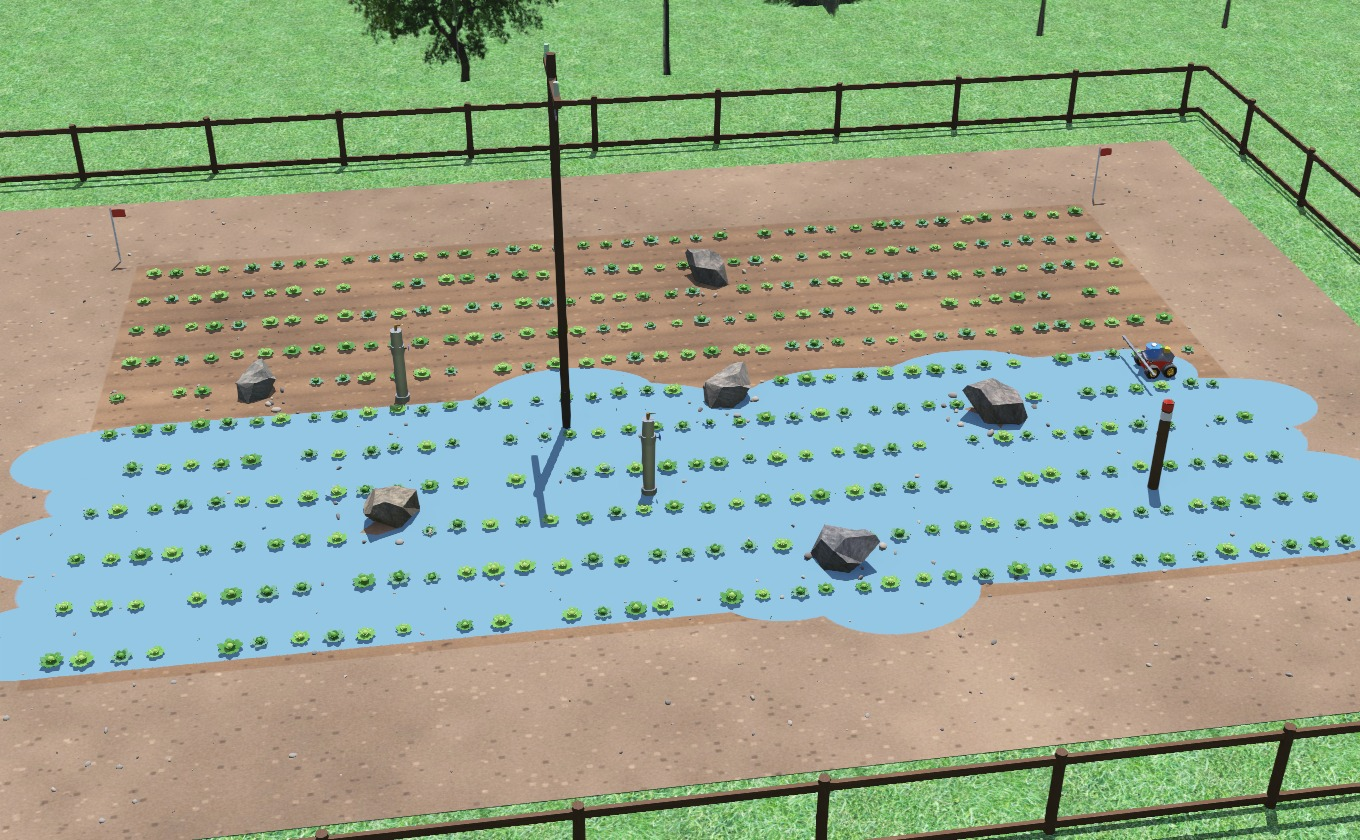
\includegraphics[width=0.92\linewidth]{figures/shot_overview.jpg}
\caption{Webots world: lettuce field with 11 crop rows, six stones and four poles. The blue area is the soil already sprayed by the robot (Pen device) after 215~s.}
\label{fig:overview}
\end{figure}

\section{Problem Statement and Objectives}
\textbf{Problem statement.} A ground robot must spray a rectangular crop field of 16~m $\times$ 10~m whose crop rows are 1.0~m apart. It must cover the field row by row (boustrophedon coverage) with a 1.2~m sprayer boom, avoid static obstacles (stones and poles) that are not known in advance and may stand directly in a lane, and log the area covered and the path length. The robot should finish the field quickly, with high coverage, without collisions and without leaving its lane pattern.

\textbf{Objectives.}
\begin{enumerate}[itemsep=0pt,topsep=2pt]
\item Build a Webots world of a crop field with headlands, crop rows, stones and poles, and equip a Pioneer~3-AT with lidar, GPS, inertial unit, sprayer boom and a live dashboard.
\item Plan a boustrophedon coverage path with two headland-turn manoeuvres (arc and pivot) and follow it with a cross-track error below 5~cm RMS.
\item Detect and map unknown obstacles with the lidar and avoid them with zero collisions while keeping at least 98\,\% coverage of the coverable area.
\item Compare the proposed detour method with at least two classical methods (Bug2, artificial potential field) on 20 random fields, and study turn type, obstacle density, boom width and controller gains.
\end{enumerate}

\textbf{Assumptions and limits.} The ground is flat; obstacles are static and roughly circular (stones 0.3--0.42~m radius, poles 0.06--0.10~m radius); GPS and inertial unit give the robot pose (no localisation drift is modelled); crop plants are lower than the lidar plane and are not physical obstacles in simulation. Ground-truth obstacle positions are used only to compute evaluation metrics, never by the robot.

\section{Literature and Industry Review}
\textbf{Coverage path planning.} Galceran and Carreras survey coverage path planning and classify it into cellular decomposition, grid-based and sensor-based methods \cite{galceran2013}. Choset's boustrophedon cellular decomposition splits a known map into cells that are each covered by back-and-forth lanes \cite{choset2000}. Oksanen and Visala adapt coverage planning to agricultural machines and show that headland turns and driving direction dominate the non-productive time \cite{oksanen2009}. Hameed et al.\ optimise the driving angle and treat known obstacle areas as separate blocks \cite{hameed2013}. These planners assume the obstacles are known before the robot starts.

\textbf{Reactive obstacle avoidance.} Khatib's artificial potential field (APF) attracts the robot to its goal and repels it from obstacles \cite{khatib1986}; Koren and Borenstein showed its inherent problems: local minima, oscillation near obstacles and in narrow passages \cite{koren1991}. The Bug family of algorithms by Lumelsky and Stepanov guarantees completeness for a point robot by following the obstacle boundary until the robot meets the line to the goal (the M-line) again \cite{lumelsky1987}. Brooks' layered (subsumption) architecture shows how such reflexes can sit below deliberative layers \cite{brooks1986}.

\textbf{Path tracking and control.} Pure pursuit steers towards a look-ahead point on the path and is the standard tracker for field vehicles \cite{coulter1992}; heading or speed loops are usually closed with PID control \cite{astrom2008}. Wheeled-robot kinematics, including skid steering, is covered in \cite{siegwart2011}.

\textbf{Industry.} Commercial and research platforms (Thorvald~II \cite{grimstad2017}, and the robots surveyed in \cite{bechar2016,vougioukas2019}) combine RTK-GNSS lane following with a safety field from lidar or cameras that \emph{stops} the vehicle; ISO~18497 defines the safety principles for such machines \cite{iso18497}. Lidar data near vegetation contain artefacts such as mixed pixels that must be filtered \cite{tuley2005}.

\textbf{Gap.} Map-based planners need prior obstacle maps, and purely reactive methods are safe but do not preserve the lane pattern, so they can lose rows or leave untreated strips. Industrial systems often simply stop. What is missing is a light-weight, sensor-based method that keeps the boustrophedon structure intact when an unknown obstacle appears, together with a quantitative comparison against the classical reactive methods. Table~\ref{tab:lit} summarises the comparison.

\begin{table}[H]
\centering
\caption{Comparison of existing approaches with this work}
\label{tab:lit}
\renewcommand{\arraystretch}{1.25}
\begin{tabular}{|P{3.5cm}|P{4.6cm}|P{5.0cm}|}
\hline
\textbf{Approach} & \textbf{Strength} & \textbf{Limitation} \\ \hline
Boustrophedon decomposition \cite{choset2000,hameed2013} & Complete, low overlap & Obstacles must be known in advance \\ \hline
APF \cite{khatib1986,koren1991} & Simple, reactive, fast & Local minima, oscillation, loses the lane \\ \hline
Bug2 boundary following \cite{lumelsky1987} & Complete for a point robot & Long loops, re-joins late, no memory \\ \hline
Industrial lane following + safety stop \cite{grimstad2017,iso18497} & Safe and certified & Stops at obstacles; needs an operator \\ \hline
\textbf{This work} & Sensor-based map, keeps the lane pattern, smooth arcs & Circular obstacle model; flat ground \\ \hline
\end{tabular}
\end{table}

\section{Novelty}
Compared with the textbook boustrophedon planner and the classical reactive methods, this project contributes the following. Each point is supported by our own results in Section~9.
\begin{enumerate}[itemsep=2pt,topsep=2pt]
\item \textbf{Lane-preserving geometric detour.} Obstacles seen by the lidar are mapped as circles, and the blocked part of the planned lane is replaced by a circular arc of radius $R=\hat r+r_{robot}+m$ that starts and ends on the \emph{same} lane, on the shorter safe side (Figure~\ref{fig:detour}). \emph{Evidence:} on 20 random fields the method finished 20 of 20 fields with 98.85\,$\pm$\,0.14\,\% coverage and never skipped a lane segment, against 95.41\,$\pm$\,2.15\,\% (11 runs with skipped segments) for Bug2 and 85.30\,$\pm$\,26.69\,\% (15 of 20 finished) for APF (Table~\ref{tab:mc}).
\item \textbf{Robust lidar mapping in a crop field.} An isolated-return (mixed-pixel) filter and an IMU-based hit-height filter remove ghost returns and crop-top hits before clustering. \emph{Evidence:} without the filters the Webots robot built 31 confirmed obstacles (17 of them phantoms) and became stuck in lane 5; with the filters it mapped only the 10 real obstacles plus the 4 corner flags and finished the field (Section~9.6).
\item \textbf{Layered agent with speed scheduling, identical in Webots and a headless simulator.} A declarative--procedural--reflexive agent (Figure~\ref{fig:arch}) slows down near obstacles and in turns. \emph{Evidence:} the same code gives 98.43\,\% coverage in Webots and 98.97\,\% in the headless simulator on the demonstration field, with zero collisions in all 126 Webots and headless runs of the proposed method.
\item \textbf{Quantitative design study for the operator.} We measured the effect of the headland turn type (arc turns are 7.4\,\% faster than pivot turns: 412 vs 443~s), boom width (1.2~m gives 98.84\,\% coverage with 23.9\,\% overlap) and obstacle density (coverage falls only from 100\,\% to 98.1\,\% from 0 to 16 obstacles), see Figures~\ref{fig:density} and \ref{fig:toolwidth}.
\item \textbf{Live coverage accounting and visualisation.} A 5~cm coverage grid counts passes per cell, the Webots Pen device paints the sprayed soil and an on-screen dashboard shows coverage, state and a coverage minimap during the run (Figure~\ref{fig:shots}).
\end{enumerate}

\section{Syllabus Mapping and Theory}
Table~\ref{tab:syllabus} maps the AISR syllabus topics to the parts of the project where they are used.

\begin{table}[H]
\centering
\caption{AISR syllabus topics used in the project}
\label{tab:syllabus}
\renewcommand{\arraystretch}{1.25}
\begin{tabular}{|P{4.2cm}|P{9.0cm}|}
\hline
\textbf{Syllabus topic} & \textbf{Where it is used} \\ \hline
Uninhabited ground robots & Pioneer~3-AT skid-steer model, wheel speed limits, sensors (lidar, GPS, IMU) \\ \hline
Path planning & Boustrophedon coverage plan, geometric detour planner, Bug2 and APF baselines \\ \hline
Planning to move & Headland manoeuvres (arc and pivot), pure-pursuit tracking, speed scheduling \\ \hline
Application domains & Precision agriculture: crop-row spraying, coverage and overlap metrics \\ \hline
Open/closed-loop control & PID heading loop, look-ahead control, step-response tuning \\ \hline
Robotic perception & Lidar scan to points, ghost filtering, clustering, circle fitting, obstacle map \\ \hline
Software architectures & Declarative--procedural--reflexive layered agent, sensor/actuator abstraction \\ \hline
\end{tabular}
\end{table}

\subsection{Robot kinematics}
The robot is modelled as a unicycle with pose $(x,y,\theta)$, forward speed $v$ and yaw rate $\omega$:
\begin{equation}
\dot x = v\cos\theta, \qquad \dot y = v\sin\theta, \qquad \dot\theta = \omega .
\end{equation}
For a skid-steer base with wheel radius $r_w=0.11$~m, the left and right wheel angular speeds are
\begin{equation}
\omega_{L,R} = \frac{v \mp \omega\, b_{\mathrm{eff}}/2}{r_w}, \qquad |\omega_{L,R}| \le 6.4~\mathrm{rad/s},
\label{eq:wheels}
\end{equation}
where $b_{\mathrm{eff}} = 1.4 \times 0.394$~m is an effective track width that accounts for wheel slip during skid steering \cite{siegwart2011}. If a wheel would saturate, both wheel speeds are scaled by the same factor so the path curvature is kept.

\subsection{Boustrophedon coverage}
For a field of width $W$ (across the rows) and lane spacing $s$, the number of lanes is $n=\lceil W/s\rceil$ with lane centres at $y_k = y_{\min} + s/2 + k s$. Each lane of length $L_r$ is extended by an overshoot $o$ at both ends so the boom covers the row ends. The planned path length is approximately
\begin{equation}
L_{\mathrm{arc}} = n(L_r+2o) + (n-1)\frac{\pi s}{2}, \qquad L_{\mathrm{pivot}} = n(L_r+2o) + (n-1)s,
\end{equation}
which gives 181.7~m (arc) and 176.7~m (pivot) for our field ($n=10$, $L_r=16$~m, $o=0.3$~m, $s=1$~m, plus the 1.7~m transit from the start).

\subsection{Pure pursuit and PID heading control}
The tracker chooses a look-ahead point $p_t$ on the path at distance $L$ from the robot and computes the heading error $e_\theta = \mathrm{wrap}(\mathrm{atan2}(y_t-y,\,x_t-x)-\theta)$. Pure pursuit would command the curvature $\kappa = 2\sin e_\theta / L$ \cite{coulter1992}. We close the loop on $e_\theta$ with a PID controller \cite{astrom2008}:
\begin{equation}
\omega = K_p e_\theta + K_i \int e_\theta\,dt + K_d \frac{de_\theta}{dt}, \qquad |\omega| \le 1.6~\mathrm{rad/s},
\end{equation}
with $K_p=2.2$, $K_i=0.05$ and $K_d=0.12$ (tuned in Section~9.5). The forward speed is scheduled as
\begin{equation}
v = v_{\max}\, s_{\mathrm{obs}}\, s_{\mathrm{turn}} \max(0,\cos e_\theta), \qquad s_{\mathrm{obs}} = \mathrm{clip}\!\left(\frac{d_f-d_{\mathrm{stop}}}{d_{\mathrm{slow}}-d_{\mathrm{stop}}},\,0.35,\,1\right),
\label{eq:speed}
\end{equation}
where $d_f$ is the smallest lidar range within $\pm30^\circ$ ahead, $d_{\mathrm{stop}}=0.4$~m, $d_{\mathrm{slow}}=2.0$~m, $v_{\max}=0.5$~m/s and $s_{\mathrm{turn}}=0.6$ in headland turns. If $|e_\theta|>55^\circ$ the robot rotates in place (pivot) until $|e_\theta|<15^\circ$.

\subsection{Obstacle geometry and detour}
A lidar cluster with end points $p_1,p_n$ at mean range $\bar\rho$ is approximated by a circle of radius $\hat r = \tfrac12(\|p_n-p_1\| + \Delta\phi\,\bar\rho)$ ($\Delta\phi$ is the angular resolution) whose centre is the cluster centroid moved $0.8\hat r$ away from the robot. The safety radius is $R=\hat r + r_{robot} + m$ with $r_{robot}=0.32$~m and margin $m=0.30$~m. A path segment $a\!\to\!b$ enters the circle $(c,R)$ at the smallest $t\in[0,1]$ that solves
\begin{equation}
\|a + t(b-a) - c\|^2 = R^2 .
\end{equation}
Between the entry point $p_e$ and exit point $p_x$ the lane is replaced by the arc $c + R(\cos\phi,\sin\phi)$, $\phi$ from $\angle(p_e-c)$ to $\angle(p_x-c)$, on the shorter of the two sides that stays inside the field and clear of other obstacles. Its length is $R\,|\Delta\phi|$.

\subsection{Baseline methods}
\textbf{APF} \cite{khatib1986}: the heading command is the direction of $F = F_{att} + F_{rep} + F_{vortex}$, with $F_{att}$ the unit vector to the look-ahead point and, for the closest return at distance $d<d_0=1.5$~m in direction $u$,
\begin{equation}
F_{rep} = -k\left(\frac1d-\frac1{d_0}\right)\frac{u}{d^2}, \qquad F_{vortex} = \|F_{rep}\|\, R_{\pm 90^\circ} u ,
\end{equation}
where the vortex term (with a locked side) is the usual remedy for APF local minima \cite{koren1991}. \textbf{Bug2} \cite{lumelsky1987}: when $d_f<0.9$~m the robot follows the obstacle boundary at 0.75~m and leaves it when it crosses its lane (the M-line) at a point further along the lane than the hit point.

\subsection{Coverage metrics}
The crop area is rasterised into 5~cm cells. While spraying, every cell within $w/2$ of the boom's swept segment (boom width $w$) is marked for the current pass. Coverage is the fraction of free (non-obstacle) cells sprayed at least once; overlap is the fraction of sprayed cells sprayed in two or more passes; the clearance is the distance from the robot circle ($r=0.30$~m) to the nearest obstacle surface.

\section{System Design}
\subsection{System architecture}
Figure~\ref{fig:arch} shows the full system. The Webots controller reads the sensors, the layered agent decides, and the wheel motors and the sprayer act. The agent has three layers in the declarative--procedural--reflexive hierarchy: the \emph{declarative} layer holds the coverage plan for the whole field; the \emph{procedural} layer tracks the path, builds the obstacle map and splices detours; and the \emph{reflexive} layer stops and backs off if anything comes closer than 0.4~m to the lidar. This follows the layered-control idea of \cite{brooks1986}.

\begin{figure}[H]
\centering
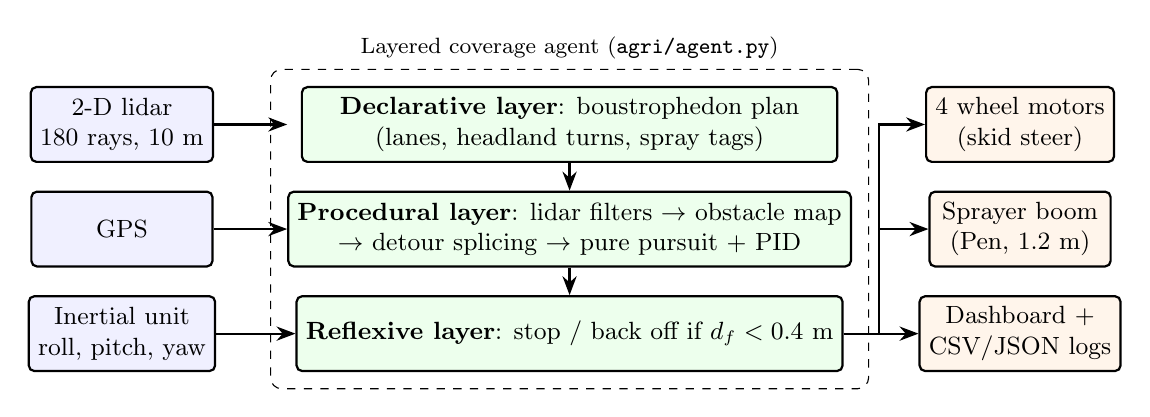
\begin{tikzpicture}[font=\small, >={Stealth[length=2.4mm]},
  box/.style={draw, thick, rounded corners=2pt, align=center, minimum height=0.95cm, fill=white},
  sens/.style={box, fill=blue!6, minimum width=2.3cm},
  act/.style={box, fill=orange!8, minimum width=2.3cm},
  lay/.style={box, fill=green!7, minimum width=6.8cm}]
\node[sens] (lidar) {2-D lidar\\180 rays, 10 m};
\node[sens, below=0.35cm of lidar] (gps) {GPS};
\node[sens, below=0.35cm of gps] (imu) {Inertial unit\\roll, pitch, yaw};
\node[lay, right=1.1cm of lidar] (dec) {\textbf{Declarative layer}: boustrophedon plan\\(lanes, headland turns, spray tags)};
\node[lay, below=0.35cm of dec] (proc) {\textbf{Procedural layer}: lidar filters $\rightarrow$ obstacle map\\$\rightarrow$ detour splicing $\rightarrow$ pure pursuit + PID};
\node[lay, below=0.35cm of proc] (refl) {\textbf{Reflexive layer}: stop / back off if $d_f<0.4$ m};
\node[act, right=1.1cm of dec] (mot) {4 wheel motors\\(skid steer)};
\node[act, below=0.35cm of mot] (pen) {Sprayer boom\\(Pen, 1.2 m)};
\node[act, below=0.35cm of pen] (dash) {Dashboard +\\CSV/JSON logs};
\begin{scope}[on background layer]
\node[draw, dashed, rounded corners, fit=(dec)(proc)(refl), inner sep=6pt, label={[font=\footnotesize]above:Layered coverage agent (\texttt{agri/agent.py})}] {};
\end{scope}
\draw[->, thick] (lidar.east) -- (proc.west |- lidar.east);
\draw[->, thick] (gps.east) -- (proc.west);
\draw[->, thick] (imu.east) -- (refl.west |- imu.east);
\draw[->, thick] (dec) -- (proc);
\draw[->, thick] (proc) -- (refl);
\draw[->, thick] (refl.east) -- ++(0.45,0) |- (mot.west);
\draw[->, thick] (refl.east) -- ++(0.45,0) |- (pen.west);
\draw[->, thick] (refl.east) -- ++(0.45,0) |- (dash.west);
\end{tikzpicture}
\caption{System architecture: sensors, layered agent and actuators}
\label{fig:arch}
\end{figure}

\subsection{Robot and environment model}
The robot is the Webots model of the Adept Pioneer~3-AT, a four-wheel-drive skid-steer platform (wheel radius 0.11~m, track 0.394~m, top wheel speed 6.4~rad/s, i.e.\ 0.70~m/s). We added to its extension slot: a single-layer lidar (180 rays over $180^\circ$, 10~m range, 1~cm noise) mounted 14.5~cm ahead of the centre at 0.35~m height, a GPS and an inertial unit, a Pen device that paints a 1.2~m wide trace on the soil while spraying, a 1.2~m sprayer boom with six nozzles, a tank and a Display used as dashboard (Figure~\ref{fig:robot}).

The world (Figures~\ref{fig:overview} and \ref{fig:farm}) is generated from a field description by the scripts in \texttt{tools/}. A 22~m $\times$ 16~m tilled-soil plot, with a generated texture of raised crop beds, wheel ruts and clods, lies inside a wooden rail fence. Around it are a farmyard with a barn, a silo, round hay bales, a parked tractor and a dirt track, and trees. Inside the plot, the 16~m $\times$ 10~m crop area has 11 rows of lettuce 1.0~m apart (about 410 plants of three varieties with natural size variation and 5\,\% missing plants), plus weeds and scattered pebbles, so the robot drives in 10 inter-row lanes. A 3~m headland is left on all sides for turning. Six stones (Webots \texttt{Rock}, 0.31--0.42~m radius, with rubble around them) and four poles (a 5.5~m wooden power pole with crossarm and insulators, two galvanised irrigation risers with valve and sprinkler, and a painted wooden marker post; 0.06--0.08~m radius) are placed by a seeded random generator. 70\,\% of the obstacles are put on a lane centre line, i.e.\ directly in the robot's way. Crops, weeds and pebbles are lower than 0.27~m and are visual only; the farmyard lies outside the plot, where lidar returns are ignored. Four corner flags mark the crop area.

\begin{figure}[H]
\centering
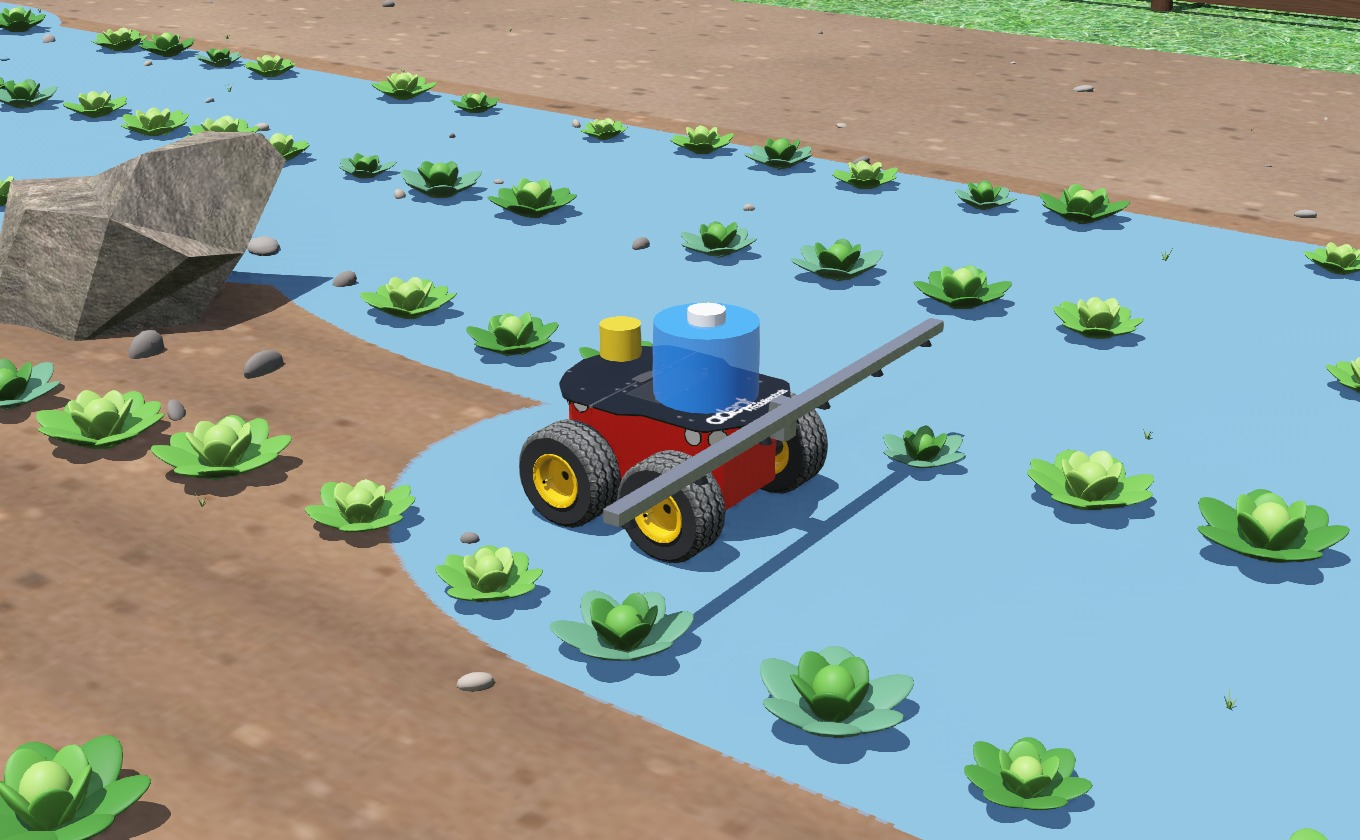
\includegraphics[width=0.5\linewidth]{figures/shot_robot.jpg}
\caption{Pioneer~3-AT with lidar (yellow), spray tank (blue) and 1.2~m sprayer boom passing a stone}
\label{fig:robot}
\end{figure}

\begin{figure}[H]
\centering
\begin{minipage}{0.53\linewidth}\centering
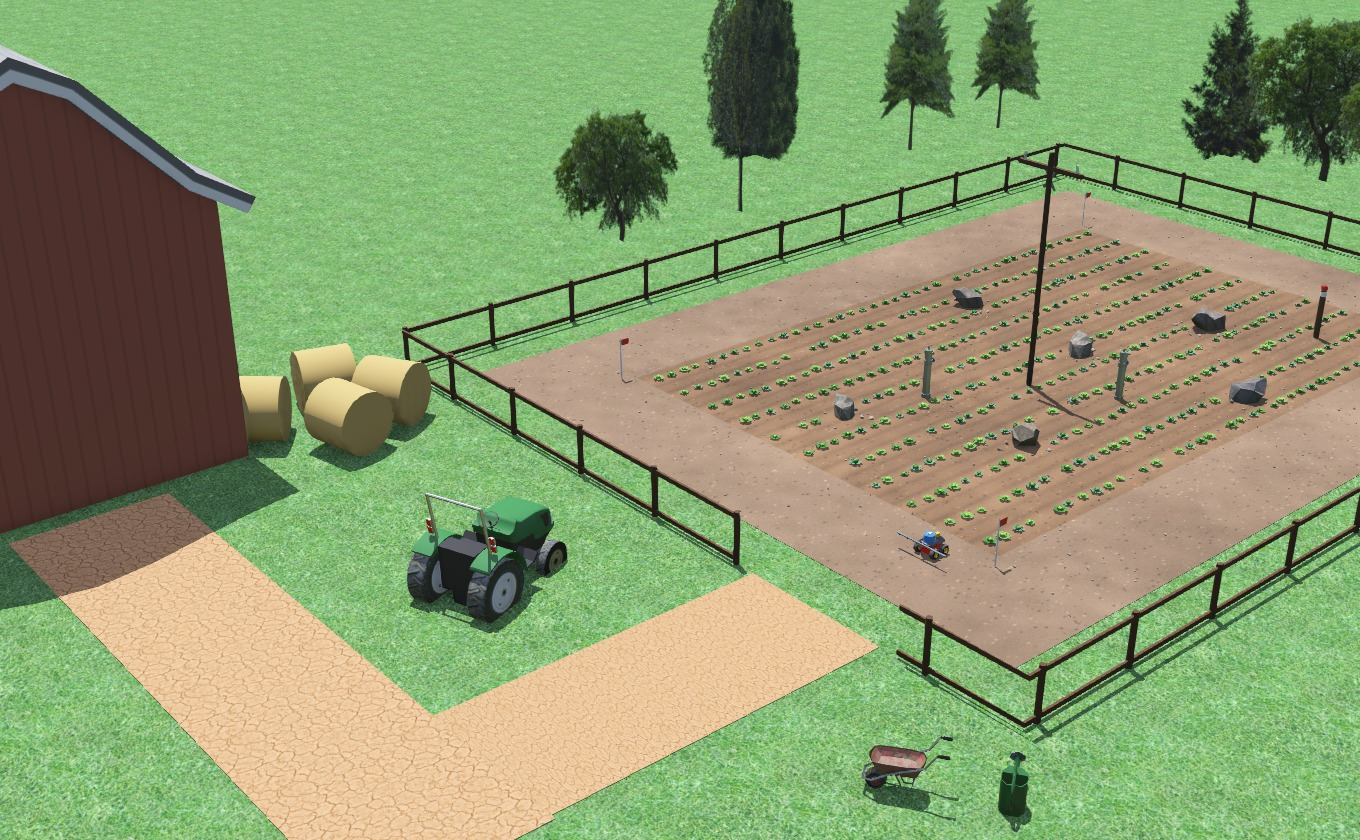
\includegraphics[width=\linewidth]{figures/shot_farm.jpg}\\[-2pt]{\footnotesize (a) farmyard and fenced field}
\end{minipage}\hfill
\begin{minipage}{0.45\linewidth}\centering
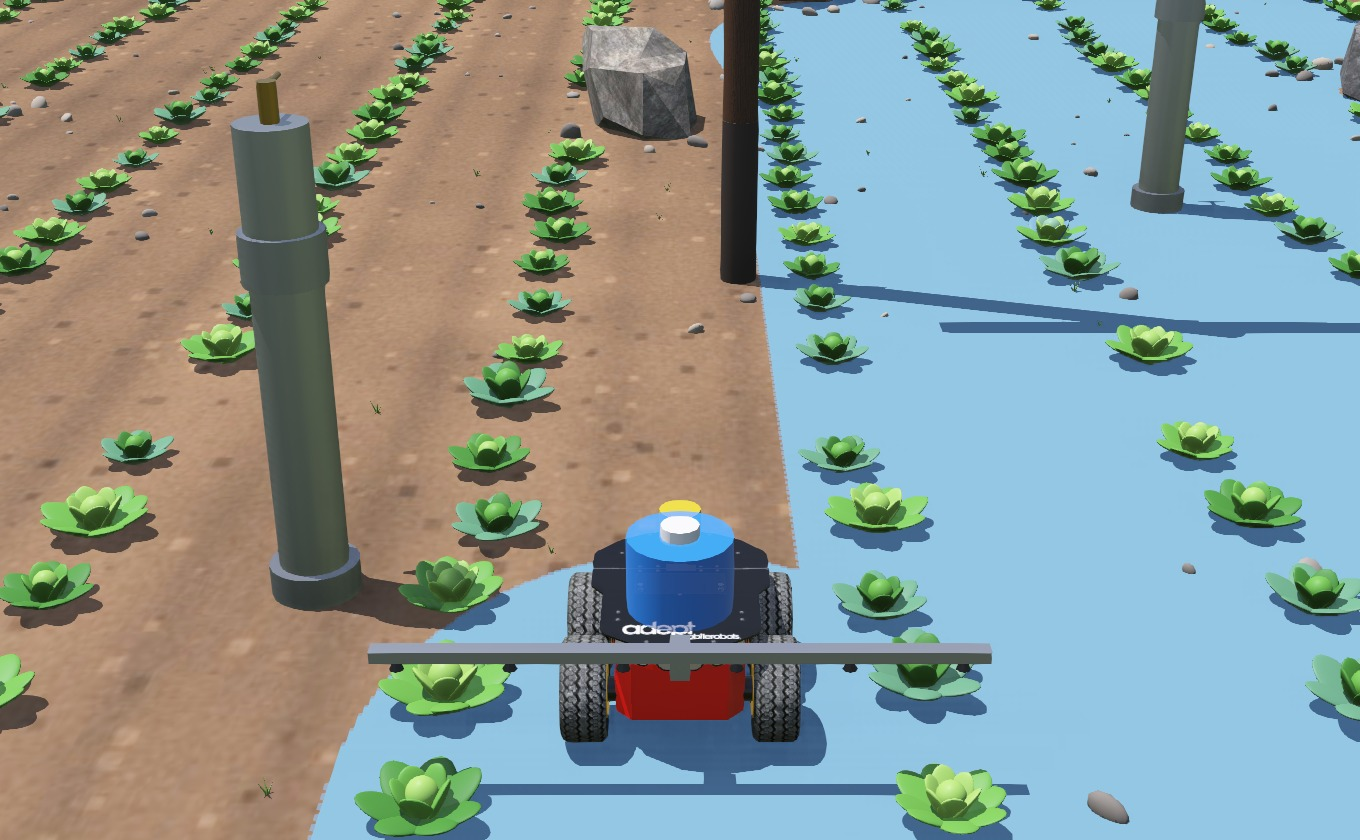
\includegraphics[width=\linewidth]{figures/shot_poles.jpg}\\[-2pt]{\footnotesize (b) irrigation riser and power pole in the rows}
\end{minipage}
\caption{Realistic environment: farmyard, lettuce rows and the pole obstacles}
\label{fig:farm}
\end{figure}

\subsection{Software architecture}
All decision making lives in the Python package \texttt{agri}, which has no Webots dependency, so exactly the same code runs in the Webots controller and in the headless simulator (Table~\ref{tab:modules}). Each module has one owner in the team (Section~10).

\begin{table}[H]
\centering
\caption{Software modules of the project repository}
\label{tab:modules}
\renewcommand{\arraystretch}{1.2}
\begin{tabular}{|P{5.9cm}|P{7.3cm}|}
\hline
\textbf{File} & \textbf{Responsibility} \\ \hline
\texttt{agri/field.py} & Field model, random field generator, JSON input/output \\ \hline
\texttt{agri/planner.py} & Boustrophedon path, arc and pivot headland turns, path splicing \\ \hline
\texttt{agri/navigation.py} & PID, pure-pursuit path tracker, speed scheduling, pivoting \\ \hline
\texttt{agri/avoidance.py} & Lidar filters, clustering, obstacle map, geometric detour, Bug2, APF \\ \hline
\texttt{agri/coverage.py} & Coverage grid, overlap, clearance, cross-track and time metrics \\ \hline
\texttt{agri/agent.py} & Layered agent that combines the modules \\ \hline
\texttt{controllers/}\newline\texttt{agri\_coverage\_controller} & Webots devices, wheel mapping, Pen, dashboard, logging, screenshots \\ \hline
\texttt{tools/generate\_world.py} & Builds the \texttt{.wbt} world, field config and soil texture \\ \hline
\texttt{sim/headless\_sim.py} & 2-D skid-steer and lidar simulator for batch runs \\ \hline
\texttt{experiments/*.py} & Monte-Carlo experiments, Webots batch runs and all figures \\ \hline
\end{tabular}
\end{table}

\section{Methodology and Algorithms}
\subsection{Control loop}
The controller runs every 32~ms (Figure~\ref{fig:flow}). It reads the GPS, inertial unit and lidar, removes low and isolated returns, updates the obstacle map, checks the path ahead for blocked segments, computes $(v,\omega)$ with the tracker, converts them into wheel speeds with Eq.~(\ref{eq:wheels}), switches the sprayer on only on lanes inside the crop area, and updates the coverage grid and logs.

\begin{figure}[H]
\centering
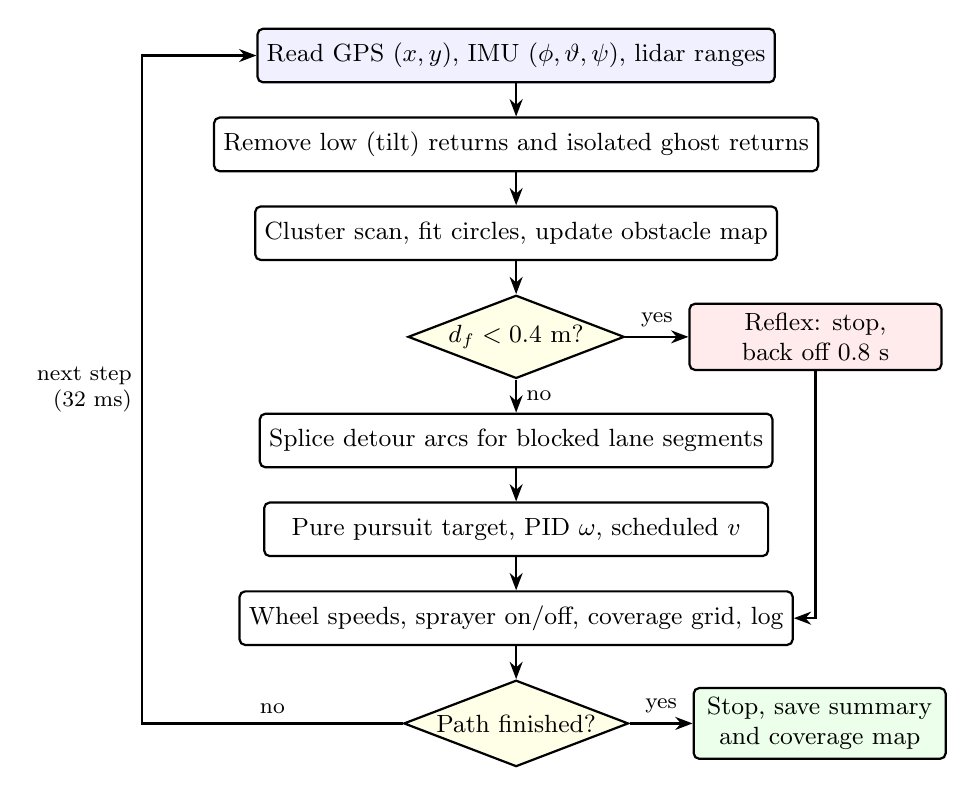
\begin{tikzpicture}[font=\small, node distance=0.42cm, >={Stealth[length=2.2mm]},
  st/.style={draw, thick, rounded corners=2pt, align=center, minimum width=6.4cm, minimum height=0.68cm, fill=white},
  dc/.style={draw, thick, diamond, aspect=2.6, align=center, inner sep=1pt, fill=yellow!10}]
\node[st, fill=blue!6] (a) {Read GPS $(x,y)$, IMU $(\phi,\vartheta,\psi)$, lidar ranges};
\node[st, below=of a] (b) {Remove low (tilt) returns and isolated ghost returns};
\node[st, below=of b] (c) {Cluster scan, fit circles, update obstacle map};
\node[dc, below=of c] (d) {$d_f < 0.4$ m?};
\node[st, right=0.8cm of d, minimum width=3.2cm, fill=red!8] (r) {Reflex: stop,\\back off 0.8 s};
\node[st, below=of d] (e) {Splice detour arcs for blocked lane segments};
\node[st, below=of e] (f) {Pure pursuit target, PID $\omega$, scheduled $v$};
\node[st, below=of f] (g) {Wheel speeds, sprayer on/off, coverage grid, log};
\node[dc, below=of g] (h) {Path finished?};
\node[st, right=0.8cm of h, minimum width=3.2cm, fill=green!8] (z) {Stop, save summary\\and coverage map};
\draw[->, thick] (a) -- (b);
\draw[->, thick] (b) -- (c);
\draw[->, thick] (c) -- (d);
\draw[->, thick] (d) -- node[above, font=\footnotesize]{yes} (r);
\draw[->, thick] (d) -- node[right, font=\footnotesize]{no} (e);
\draw[->, thick] (e) -- (f);
\draw[->, thick] (f) -- (g);
\draw[->, thick] (g) -- (h);
\draw[->, thick] (h) -- node[above, font=\footnotesize]{yes} (z);
\draw[->, thick] (h.west) -- node[above, font=\footnotesize]{no} ([xshift=-0.9cm]b.west |- h.west) |- node[left, font=\footnotesize, pos=0.25, align=right]{next step\\(32 ms)} (a.west);
\draw[->, thick] (r.south) |- (g.east);
\end{tikzpicture}
\caption{Flowchart of one control step of the coverage agent}
\label{fig:flow}
\end{figure}

\subsection{Coverage planning}
Algorithm~\ref{alg:plan} builds the dense path (one point every 0.2~m). Every point carries a lane tag ($-1$ for turns, so the sprayer is off), a corner flag for pivot vertices and a detour flag. Figure~\ref{fig:plan} shows both turn types.

\begin{algorithm}[H]
\caption{Boustrophedon coverage path with headland turns}
\label{alg:plan}
\begin{algorithmic}[1]
\Require field rectangle, lane spacing $s$, overshoot $o$, turn type
\Ensure dense path $P$ with lane tags
\State $P \gets$ straight transit from the start pose to $(x_{\min}-o,\, y_0)$, tag $-1$
\For{$k = 0 \dots n-1$}
  \State $(x_a,x_b) \gets (x_{\min}-o,\, x_{\max}+o)$ if $k$ even, else reversed
  \State append lane $(x_a,y_k)\to(x_b,y_k)$ with tag $k$
  \If{$k<n-1$}
    \If{turn = arc} append semicircle of radius $s/2$ outside the crop area, tag $-1$
    \Else\ append side-step $(x_b,y_k)\to(x_b,y_{k+1})$, mark both ends as pivot corners
    \EndIf
  \EndIf
\EndFor
\end{algorithmic}
\end{algorithm}

\begin{figure}[H]
\centering
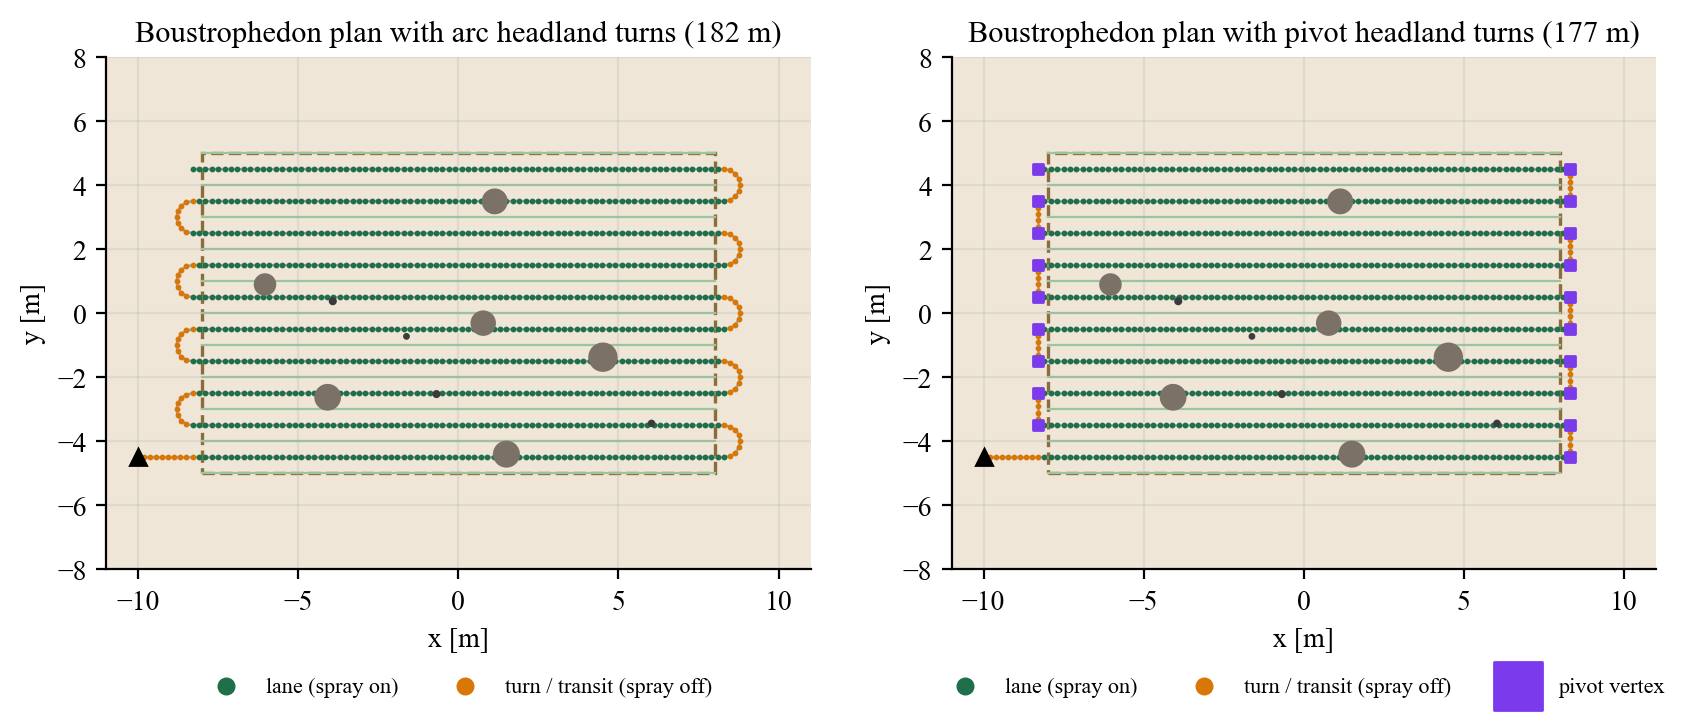
\includegraphics[width=\linewidth]{figures/fig_plan_turns.png}
\caption{Planned boustrophedon paths with arc (left) and pivot (right) headland turns}
\label{fig:plan}
\end{figure}

\subsection{Lidar perception and obstacle map}
Algorithm~\ref{alg:map} turns each scan into map updates. Two filters run first. (1) The \emph{tilt filter} computes the height of each return, $z = h - \rho\sin\vartheta\cos\alpha + \rho\cos\vartheta\sin\varphi\sin\alpha$ (lidar height $h$, pitch $\vartheta$, roll $\varphi$, bearing $\alpha$), and drops returns below 0.27~m, i.e.\ crop tops or soil hit when the body tilts. (2) The \emph{isolated-return filter} keeps a ray only if a neighbouring ray reports a similar range ($|\Delta\rho| < 0.08 + 0.06\rho$); this removes the ``mixed pixel'' ghosts that appear at object edges \cite{tuley2005}. A map entry is used for planning only after 8 consistent observations, and overlapping entries are merged into one enclosing circle. Figure~\ref{fig:perception} shows a real Webots scan.

\begin{algorithm}[H]
\caption{Lidar obstacle mapping (every control step)}
\label{alg:map}
\begin{algorithmic}[1]
\Require ranges $\rho_i$, bearings $\alpha_i$, pose, roll, pitch, map $\mathcal{M}$
\State drop returns with hit height $z_i<0.27$ m; drop isolated returns
\State $p_i \gets$ lidar origin $+\rho_i(\cos(\theta+\alpha_i),\sin(\theta+\alpha_i))$; keep points on the field soil
\State split consecutive points into clusters where $\|p_{i+1}-p_i\|>0.3$ m; skip clusters cut by the field of view
\For{each cluster} fit circle $(\hat c,\hat r)$
  \If{an entry of $\mathcal{M}$ is within $\max(0.5,\, r+\hat r+0.1)$} update it (moving average, keep $r_{\max}$)
  \Else\ add a new entry with one hit
  \EndIf
\EndFor
\State merge entries whose circles overlap; \Return confirmed entries (hits $\ge 8$)
\end{algorithmic}
\end{algorithm}

\begin{figure}[H]
\centering
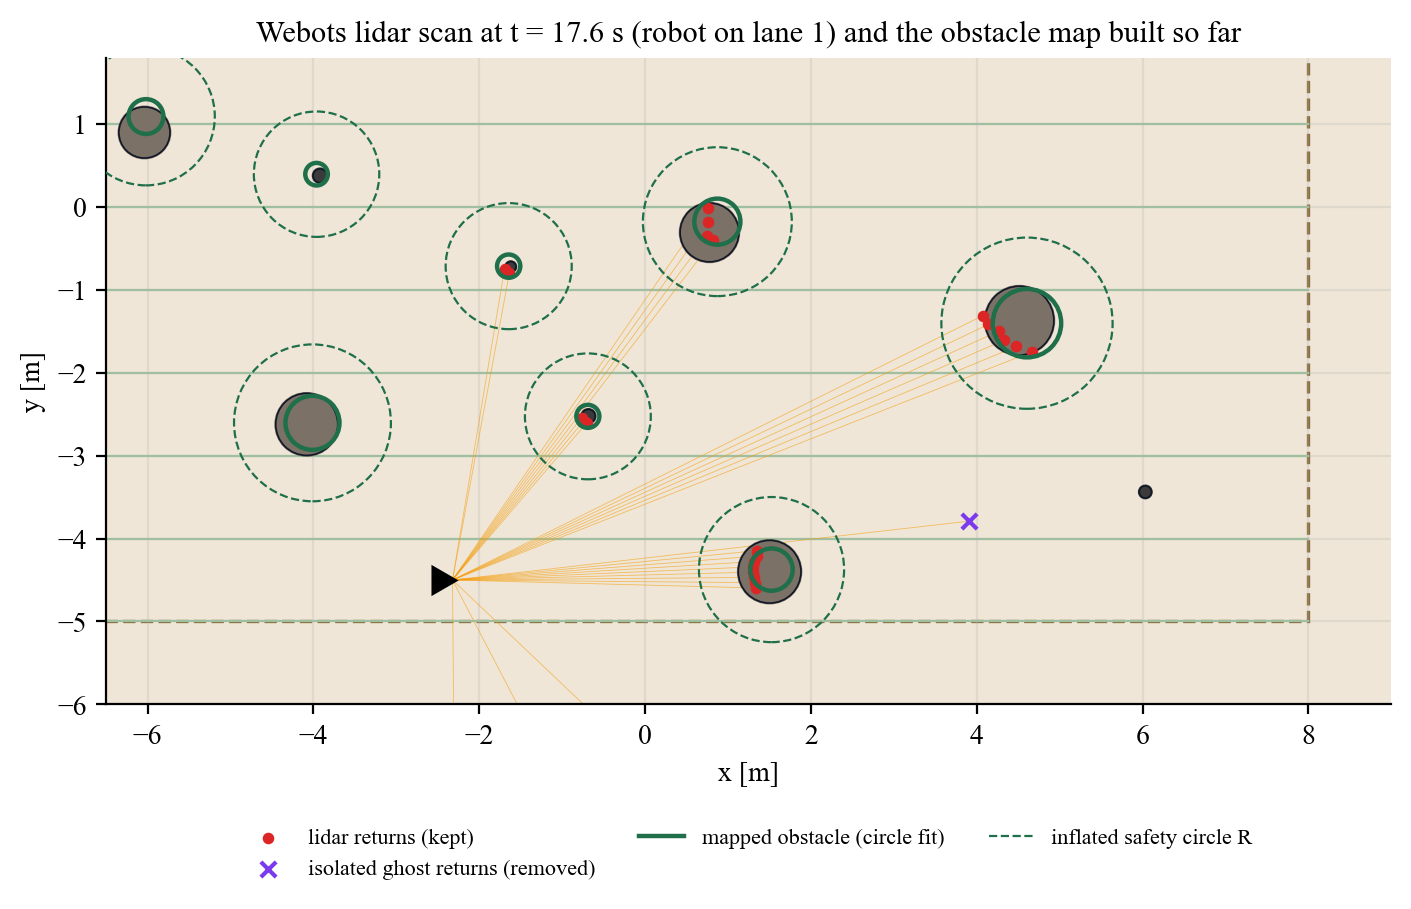
\includegraphics[width=0.95\linewidth]{figures/fig_perception.png}
\caption{Real Webots lidar scan and the obstacle map (green circles) with safety circles $R$ (dashed); black outlines are the true obstacles}
\label{fig:perception}
\end{figure}

\subsection{Geometric detour (proposed method)}
Every control step, each confirmed obstacle within the 5~m horizon is checked against the next part of the path (Algorithm~\ref{alg:detour}). If any path point lies inside $R-0.08$~m, the blocked segment is replaced by an arc (Figure~\ref{fig:detour}). The 8~cm tolerance avoids re-planning on small changes of the estimate, but a detour is re-planned if the obstacle estimate grows. While the robot drives on a detour the look-ahead is shortened from 0.6~m to 0.35~m, because pure pursuit cuts the inside of curves by about $L^2/(2R)$; this raised the minimum clearance in Webots from 1.8~cm to about 11~cm.

\begin{algorithm}[H]
\caption{Detour splicing for one mapped obstacle $(c,\hat r)$}
\label{alg:detour}
\begin{algorithmic}[1]
\State $R \gets \hat r + r_{robot} + m$; \textbf{if} robot already inside $R$ \textbf{then return} \Comment{reflex layer handles it}
\State find the first path index $i_{in}$ ahead of the robot with $\|P_i - c\|<R-0.08$; \textbf{if} none \textbf{return}
\State move $i_{in}$ back and $i_{out}$ forward while points are inside $R$
\State $p_e \gets$ entry intersection on $(P_{i_{in}-1},P_{i_{in}})$; $p_x \gets$ exit intersection on $(P_{i_{out}},P_{i_{out}+1})$
\For{direction $\in$ \{counter-clockwise, clockwise\}}
  \State build arc from $p_e$ to $p_x$ around $c$ with radius $R$ (0.2 m spacing)
  \State keep the arc if it stays on the soil and outside every other obstacle's $\hat r + r_{robot}$
\EndFor
\If{no arc is valid} replace the blocked part by $[p_e,p_x]$ and count a skip
\Else\ replace $P_{i_{in}\dots i_{out}}$ by the shorter valid arc, keeping the lane tag (sprayer stays on)
\EndIf
\end{algorithmic}
\end{algorithm}

\begin{figure}[H]
\centering
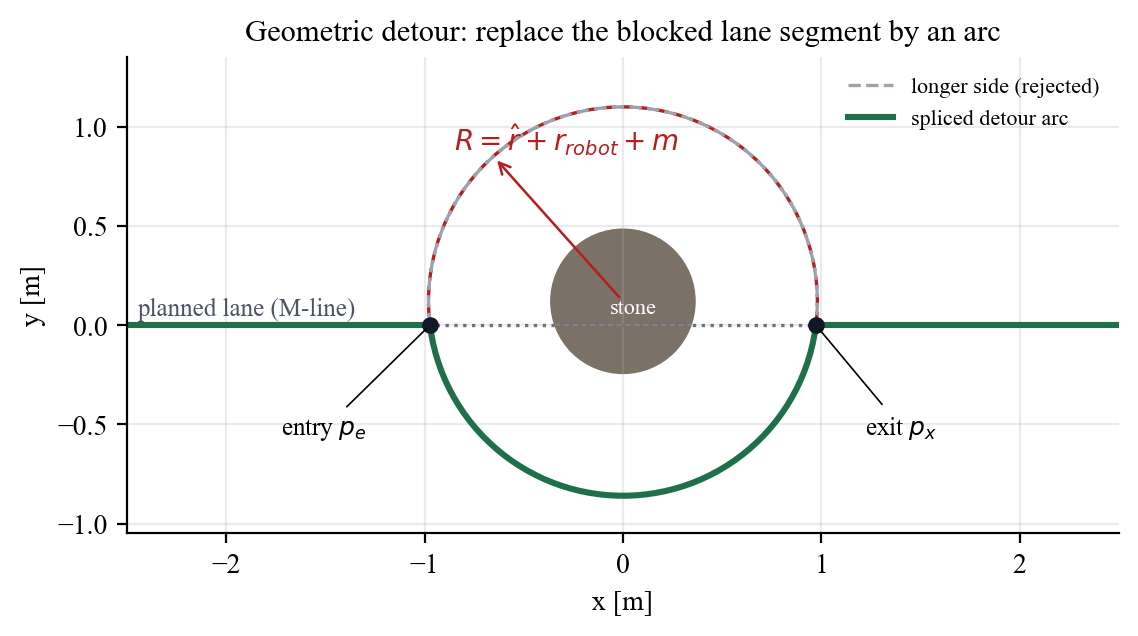
\includegraphics[width=0.78\linewidth]{figures/fig_detour_geometry.png}
\caption{Geometry of the lane-preserving detour}
\label{fig:detour}
\end{figure}

\subsection{Controller design and tuning}
The heading PID was tuned on a lateral step test: the robot starts 40~cm beside a straight lane and must converge onto it. A low gain ($K_p=1$) converges slowly and overshoots by 12.7\,\%; a high proportional gain without damping ($K_p=4.5$) saturates the yaw rate and then creeps in. The chosen gains ($K_p=2.2$, $K_i=0.05$, $K_d=0.12$) give the fastest settling (2.9~s) with negligible overshoot (Section~9.5). The small integral term removes the steady offset caused by wheel slip; its integral is clamped at $\pm0.5$ to avoid wind-up during pivots. The pivot threshold ($55^\circ$ on, $15^\circ$ off) gives hysteresis, and near $\pm180^\circ$ the pivot direction is locked to avoid chattering between left and right turns.

\section{Simulation Setup}
\textbf{Platforms.} Webots R2025a (ODE physics, 32~ms basic time step) with a Python~3 controller; the headless simulator uses the same unicycle model with wheel saturation, a first-order actuator lag ($\tau=0.12$~s), 2\,\% slip noise and a ray-casting lidar with 1~cm noise. Table~\ref{tab:params} lists the parameters.

\begin{table}[H]
\centering
\caption{Simulation and algorithm parameters}
\label{tab:params}
\renewcommand{\arraystretch}{1.15}
\begin{tabular}{|P{6.3cm}|P{6.9cm}|}
\hline
\textbf{Parameter} & \textbf{Value} \\ \hline
Crop area / soil plot & 16 m $\times$ 10 m / 22 m $\times$ 16 m (3 m headland) \\ \hline
Crop rows / lanes / lane spacing & 11 rows / 10 lanes / 1.0 m \\ \hline
Obstacles (demo field, seed 11) & 6 stones, 4 poles; coverable area 157.4 m$^2$ \\ \hline
Sprayer boom width & 1.2 m (study: 1.0--1.4 m) \\ \hline
Max speed / turn speed & 0.5 m/s / 0.3 m/s \\ \hline
Look-ahead (lane / detour / corner) & 0.6 m / 0.35 m / 0.25 m \\ \hline
PID gains $K_p, K_i, K_d$ & 2.2, 0.05, 0.12; $|\omega|\le1.6$ rad/s \\ \hline
Lidar & 180 rays, $180^\circ$, 10 m, 1 cm noise, 0.35 m high \\ \hline
Detour: $r_{robot}$, margin, horizon & 0.32 m, 0.30 m, 5 m; confirmation 8 hits \\ \hline
Reflex stop distance / slow-down distance & 0.4 m / 2.0 m \\ \hline
Coverage grid resolution & 5 cm \\ \hline
Monte-Carlo fields & 20 seeds (1--20), 6 stones + 4 poles each \\ \hline
\end{tabular}
\end{table}

\textbf{How to run.} The commands below are also in the repository README.
\begin{itemize}[itemsep=0pt,topsep=2pt]
\item Live demo: open \texttt{worlds/crop\_field.wbt} in Webots and press Run. The controller arguments in the world file select the method (\texttt{proposed}, \texttt{bug2} or \texttt{apf}) and the turn type (\texttt{arc} or \texttt{pivot}).
\item New field: \texttt{python tools/generate\_world.py --seed 3 --stones 8 --poles 5}
\item Webots batch runs (no rendering): \texttt{python experiments/run\_webots.py}
\item Headless run with plot: \texttt{python sim/headless\_sim.py --method bug2 --seed 7 --plot}
\item All statistics: \texttt{python experiments/run\_experiments.py}
\item All figures: \texttt{python experiments/make\_figures.py}
\end{itemize}

\section{Results and Analysis}
\subsection{Webots validation on the demonstration field}
Table~\ref{tab:webots} and Figure~\ref{fig:webots} compare the three avoidance methods in Webots on the same field (seed 11). All six runs finished the field without collisions. The proposed method gave the highest coverage (98.43\,\%) and the shortest time (414.6~s with arc turns). Bug2 kept the largest clearance but made full loops around two obstacles and missed 7.07~m$^2$, mainly a strip in lane 3 that it skipped when it rejoined the wrong part of the path. APF finished this field, but passed within 2.1~cm of a stone and needed 39 avoidance episodes for 10 obstacles because it oscillated.

\begin{table}[H]
\centering
\caption{Webots results on the demonstration field (6 stones, 4 poles)}
\label{tab:webots}
\renewcommand{\arraystretch}{1.2}
\small\begin{tabular}{|l|c|c|c|c|c|c|}
\hline
\textbf{Method / turns} & \textbf{Cov. [\%]} & \textbf{Overl. [\%]} & \textbf{Time [s]} & \textbf{Path [m]} & \textbf{Clear. [m]} & \textbf{Coll.} \\ \hline
Proposed / arc & \textbf{98.43} & 25.2 & \textbf{414.6} & 183.7 & 0.109 & 0 \\ \hline
Proposed / pivot & 98.42 & 25.2 & 443.7 & 182.2 & 0.083 & 0 \\ \hline
Bug2 / arc & 95.51 & 31.1 & 449.0 & 192.3 & 0.212 & 0 \\ \hline
Bug2 / pivot & 95.51 & 31.1 & 478.1 & 190.8 & 0.210 & 0 \\ \hline
APF / arc & 97.74 & 24.3 & 431.4 & 182.5 & 0.021 & 0 \\ \hline
APF / pivot & 97.80 & 24.2 & 466.5 & 180.6 & 0.020 & 0 \\ \hline
\end{tabular}
\end{table}

\begin{figure}[H]
\centering
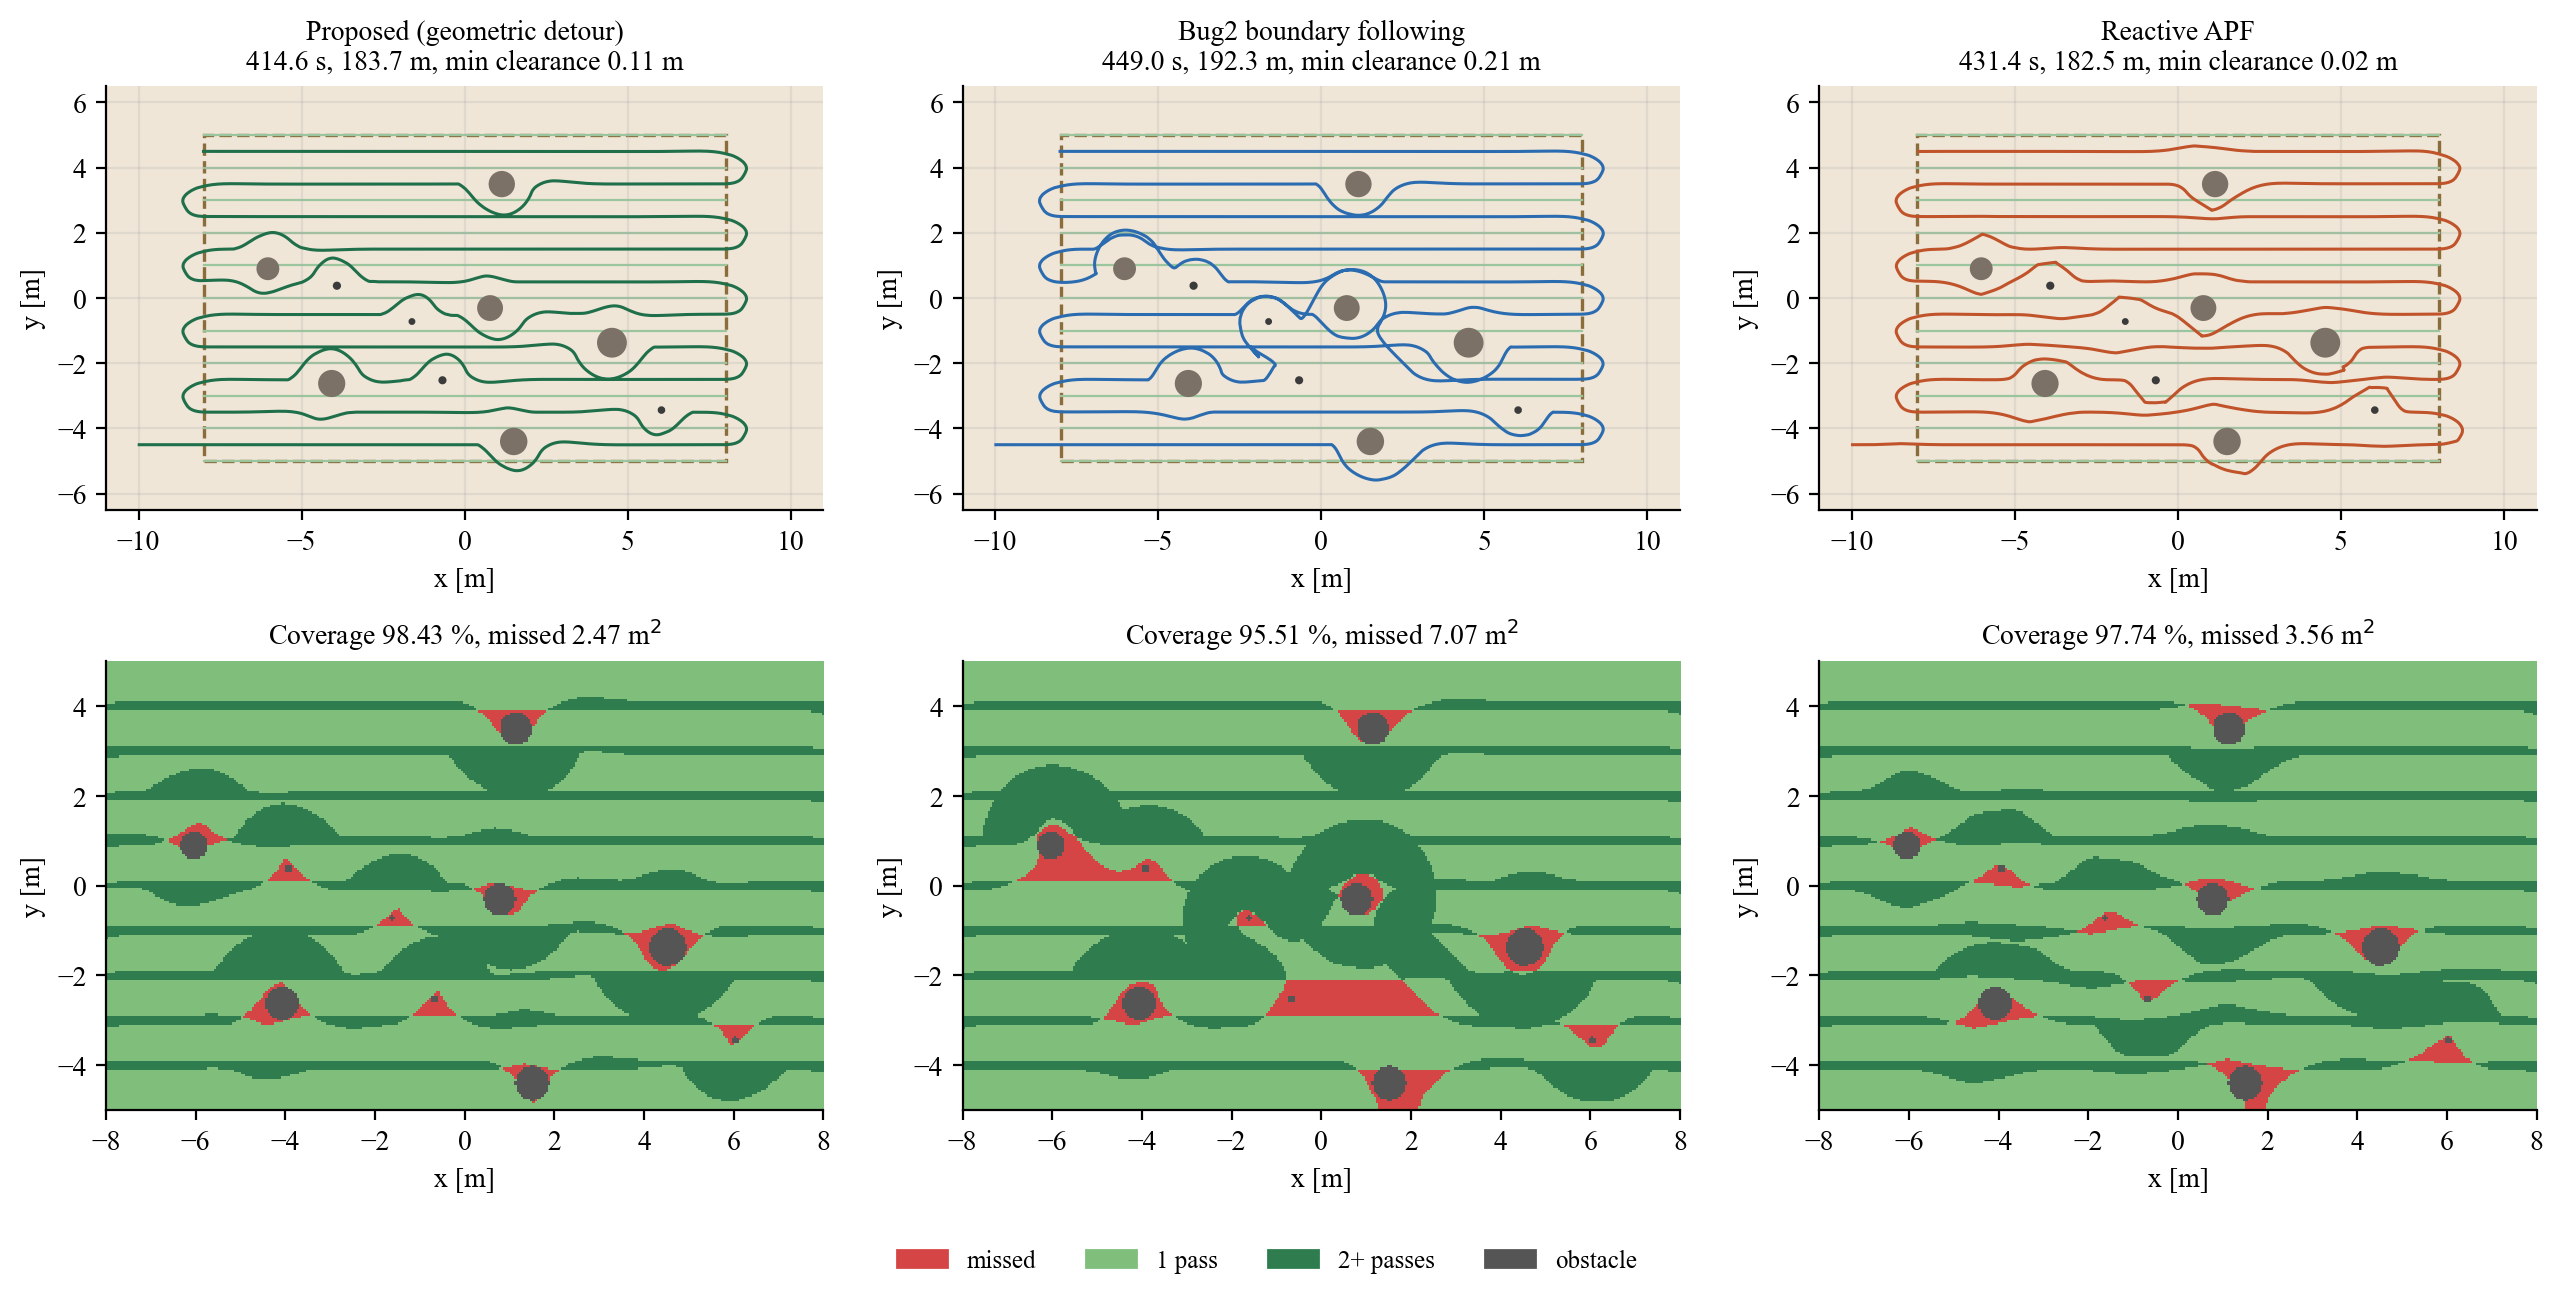
\includegraphics[width=\linewidth]{figures/fig_webots_traj.png}
\caption{Webots trajectories (top) and coverage maps (bottom) for the three methods with arc turns}
\label{fig:webots}
\end{figure}

\begin{figure}[H]
\centering
\begin{minipage}{0.49\linewidth}\centering
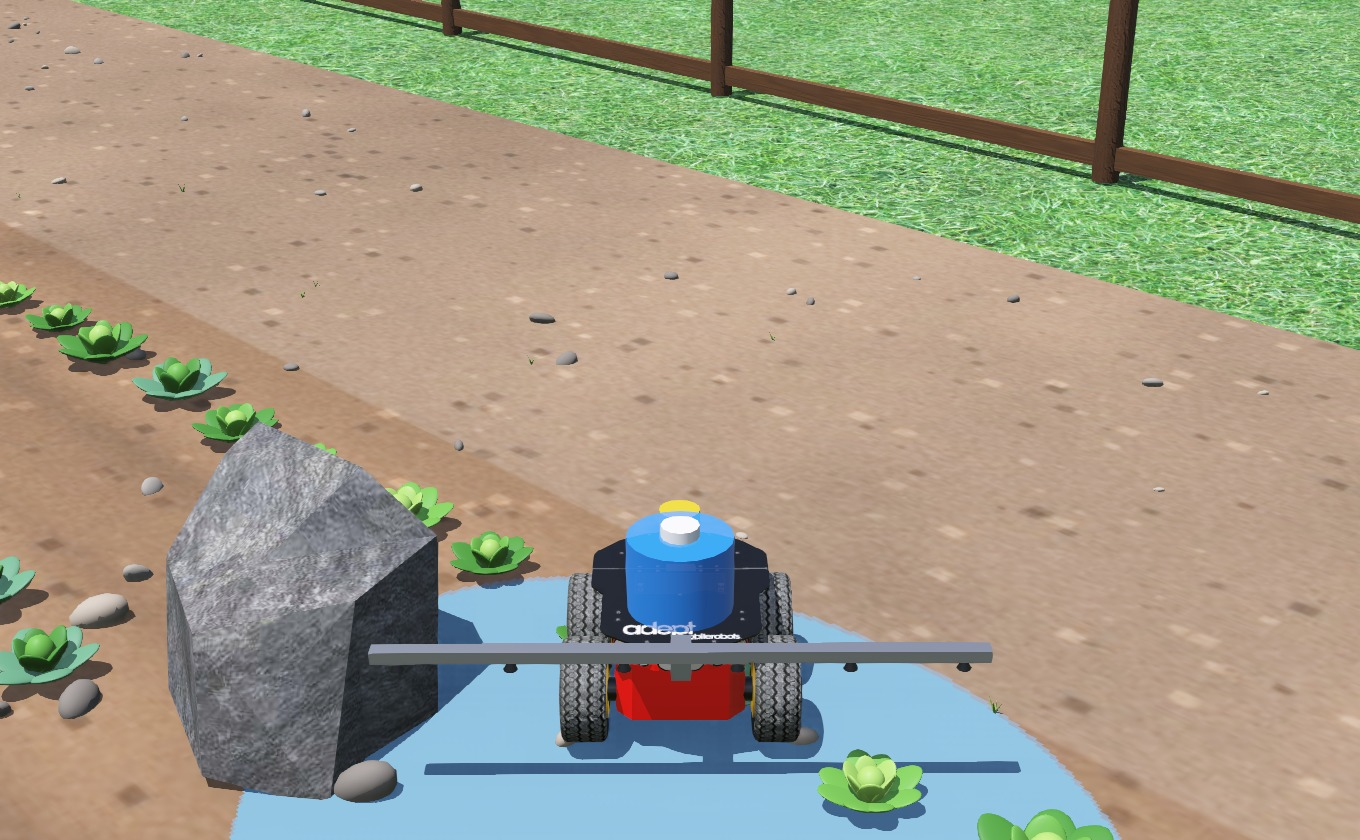
\includegraphics[width=\linewidth]{figures/shot_follow.jpg}\\[-2pt]{\footnotesize (a) approaching a stone on lane 1}
\end{minipage}\hfill
\begin{minipage}{0.49\linewidth}\centering
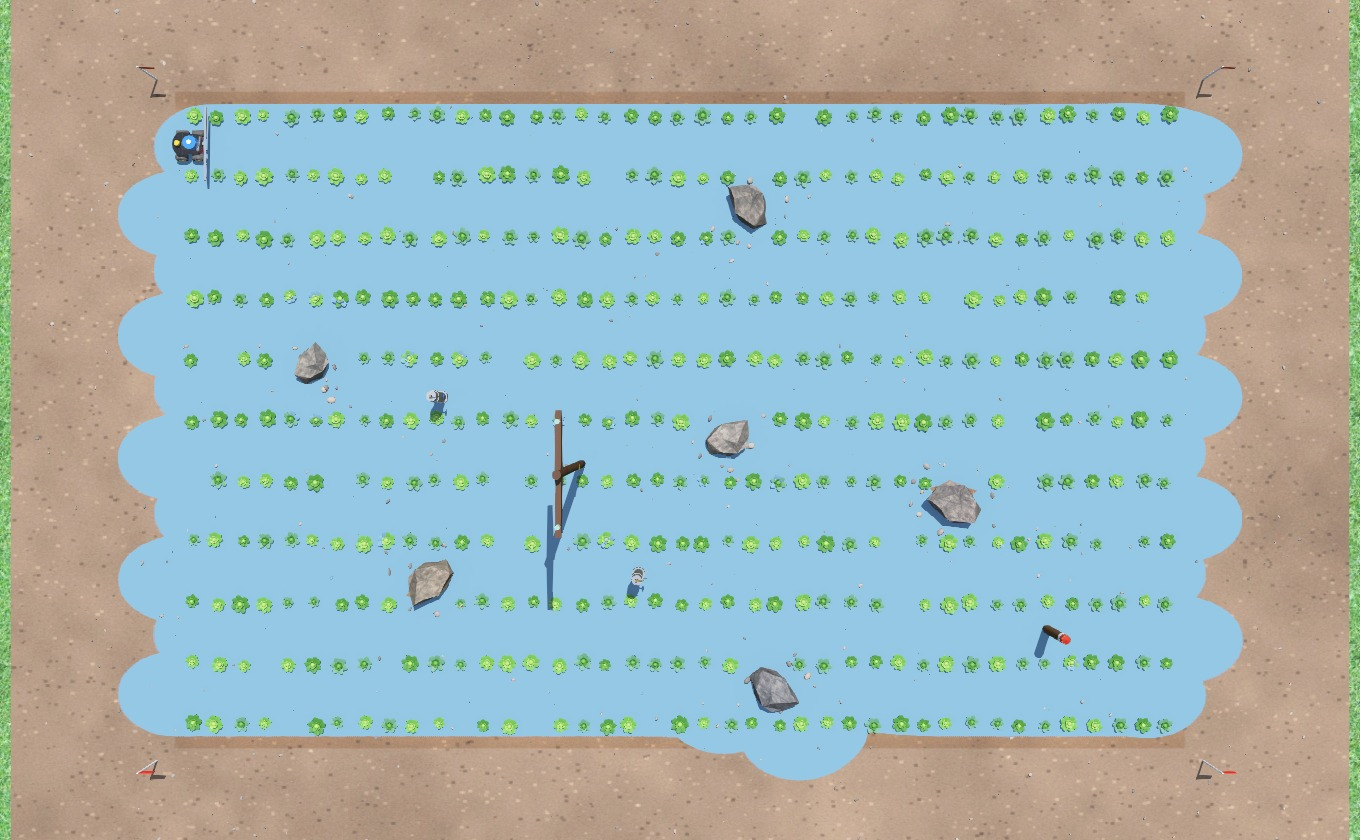
\includegraphics[width=\linewidth]{figures/shot_top_proposed.jpg}\\[-2pt]{\footnotesize (b) field painted by the sprayer after the run}
\end{minipage}\\[4pt]
\begin{minipage}{0.49\linewidth}\centering
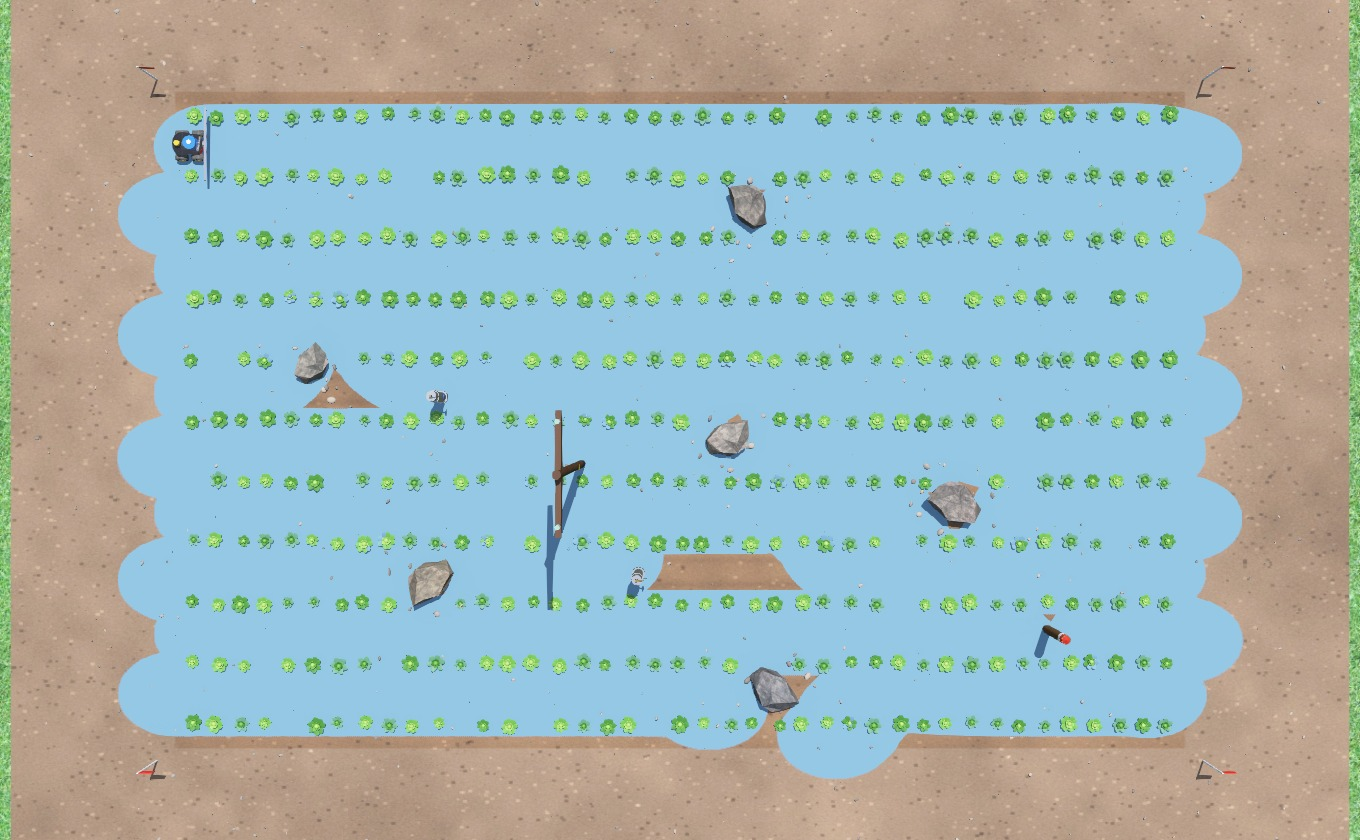
\includegraphics[width=\linewidth]{figures/shot_top_bug2.jpg}\\[-2pt]{\footnotesize (c) Bug2: unsprayed strip and gaps behind obstacles}
\end{minipage}\hfill
\begin{minipage}{0.49\linewidth}\centering
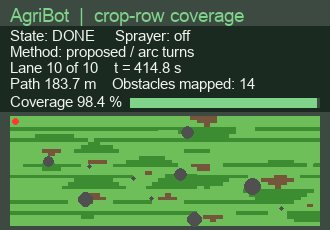
\includegraphics[width=0.78\linewidth]{figures/shot_dashboard.png}\\[-2pt]{\footnotesize (d) live dashboard at the end of the run}
\end{minipage}
\caption{Webots screenshots of the proposed method and the Bug2 baseline}
\label{fig:shots}
\end{figure}

\subsection{Monte-Carlo comparison on 20 random fields}
To test that the result is not specific to one field, each method was run on 20 random fields with both turn types in the headless simulator (120 runs, Table~\ref{tab:mc}, Figure~\ref{fig:mc}). The proposed method finished all 20 fields with almost constant coverage (98.85\,$\pm$\,0.14\,\%, worst 98.52\,\%), constant time (412\,$\pm$\,2~s) and a cross-track error of only 2.1~cm RMS. Bug2 also finished all fields but skipped part of a lane in 11 of 20 fields, which lowered coverage to 95.41\,\% on average and 89.78\,\% in the worst field; its loops made it 14\,\% slower. APF failed to finish 5 of 20 fields within the 1500~s limit because it became trapped in limit cycles near obstacles close to the headland. Its clearance was the smallest (0.124~m on average) and its cross-track error was 13 times larger. No method collided in any run.

\begin{table}[H]
\centering
\caption{Monte-Carlo results on 20 random fields, arc turns (mean $\pm$ standard deviation)}
\label{tab:mc}
\renewcommand{\arraystretch}{1.2}
\begin{tabular}{|P{4.4cm}|C{2.8cm}|C{2.8cm}|C{2.8cm}|}
\hline
\textbf{Metric} & \textbf{Proposed} & \textbf{Bug2} & \textbf{APF} \\ \hline
Fields finished & \textbf{20 / 20} & 20 / 20 & 15 / 20 \\ \hline
Coverage [\%] & \textbf{98.85 $\pm$ 0.14} & 95.41 $\pm$ 2.15 & 85.30 $\pm$ 26.69 \\ \hline
Worst-case coverage [\%] & \textbf{98.52} & 89.78 & 13.32 \\ \hline
Missed area [m$^2$] & \textbf{1.81} & 7.23 & 23.12 \\ \hline
Completion time [s] & \textbf{412.3 $\pm$ 1.6} & 471.5 $\pm$ 49.6 & 780.6 $\pm$ 437.1 \\ \hline
Path length [m] & \textbf{181.7 $\pm$ 0.4} & 207.2 $\pm$ 21.8 & 258.1 $\pm$ 93.3 \\ \hline
Minimum clearance [m] & 0.215 $\pm$ 0.014 & \textbf{0.228 $\pm$ 0.028} & 0.124 $\pm$ 0.007 \\ \hline
RMS cross-track error [cm] & \textbf{2.1 $\pm$ 0.1} & 11.3 $\pm$ 9.5 & 28.3 $\pm$ 15.3 \\ \hline
Runs with skipped segments & \textbf{0} & 11 & 19 \\ \hline
Collisions (total) & 0 & 0 & 0 \\ \hline
\end{tabular}
\end{table}

\begin{figure}[H]
\centering
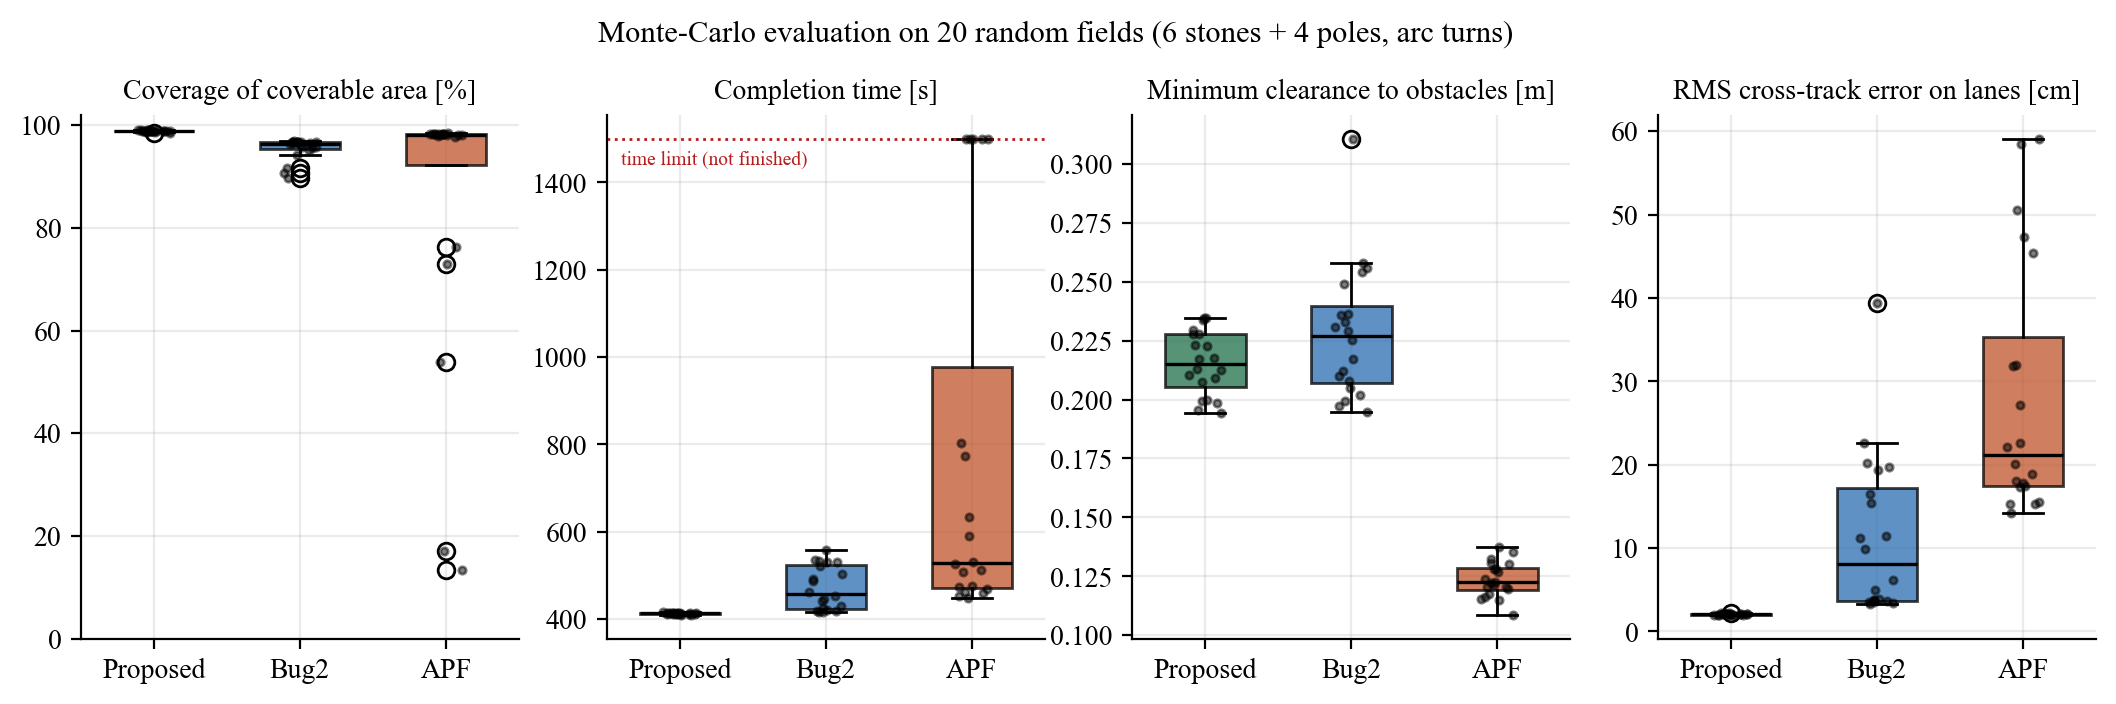
\includegraphics[width=\linewidth]{figures/fig_mc_box.png}
\caption{Distribution of coverage, time, clearance and cross-track error over 20 random fields}
\label{fig:mc}
\end{figure}

\subsection{Arc versus pivot headland turns}
Pivot turns plan a 5~m shorter path (176.7 vs 181.7~m) but stop the robot twice per turn to rotate in place. Over 20 fields the proposed method needed 412.3~s with arc turns and 442.8~s with pivot turns, so arc turns are 7.4\,\% faster for the same coverage (98.85 vs 98.83\,\%). Pivot turns gave a slightly lower lane cross-track error (1.4 vs 2.1~cm RMS) because the robot enters each lane already aligned. For a skid-steer robot with a 1~m lane spacing we therefore recommend arc turns; pivot turns are useful when the headland is narrower than the lane spacing.

\subsection{Effect of obstacle density and boom width}
Figure~\ref{fig:density} shows ten fields for each obstacle count from 0 to 16. Without obstacles all methods are identical (100\,\%, 369~s). With more obstacles the proposed method degrades gracefully: coverage drops to 98.1\,\% and time rises by only 18\,\% at 16 obstacles. Bug2 drops to 91.5--92.9\,\% and becomes 70\,\% slower at 12--16 obstacles, when obstacles are close enough to each other that its boundary loops interact.

\begin{figure}[H]
\centering
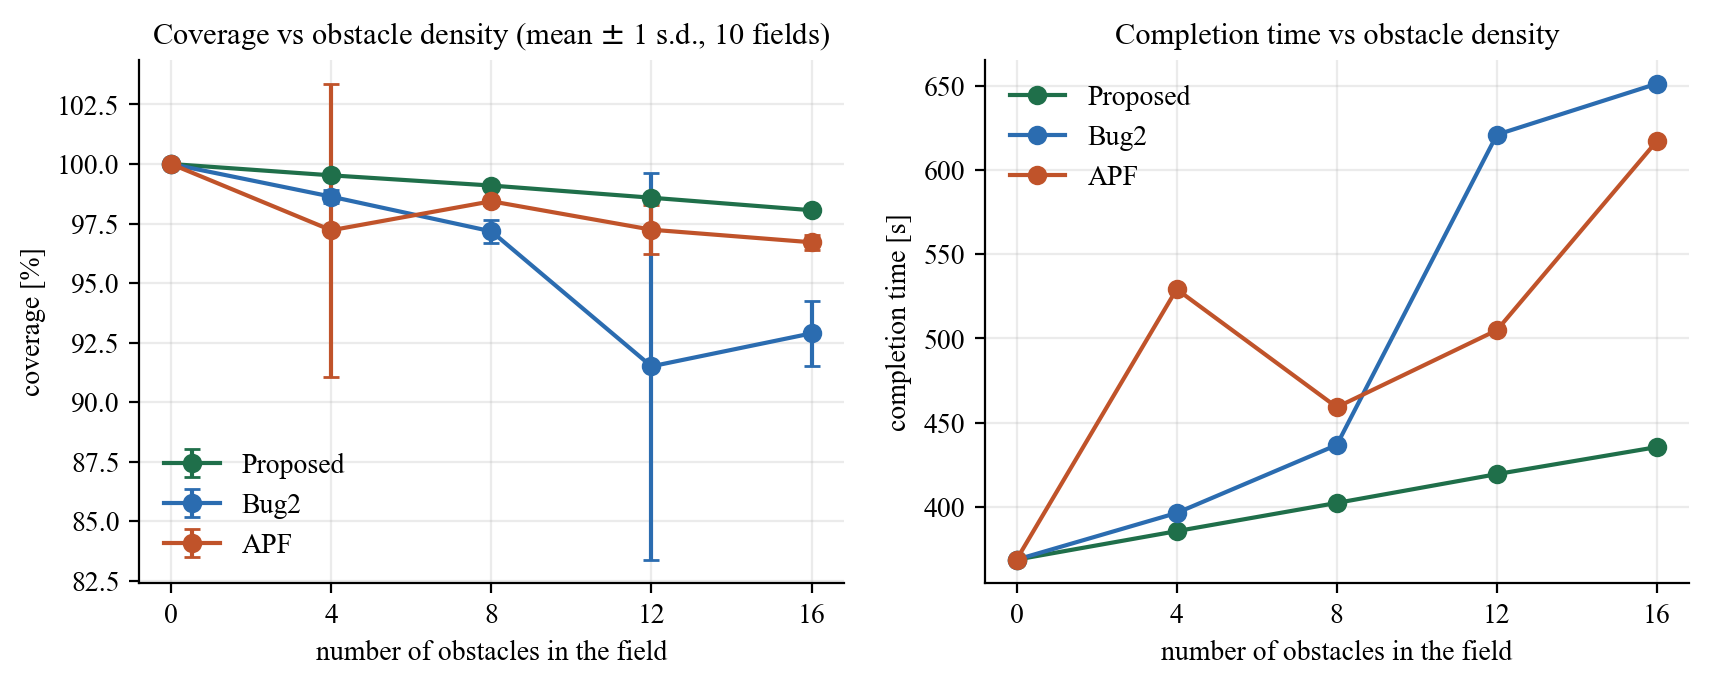
\includegraphics[width=\linewidth]{figures/fig_density.png}
\caption{Coverage and completion time versus the number of obstacles}
\label{fig:density}
\end{figure}

The boom width trades coverage against chemical overlap (Figure~\ref{fig:toolwidth}, Table~\ref{tab:tool}). With 1.0~m lanes, a boom of exactly 1.0~m leaves strips at every small tracking error (96.36\,\%), while 1.4~m almost removes misses but sprays 40.5\,\% of the area twice. The chosen 1.2~m boom gives 98.84\,\% coverage with 23.9\,\% overlap.

\begin{figure}[H]
\centering
\begin{minipage}{0.56\linewidth}
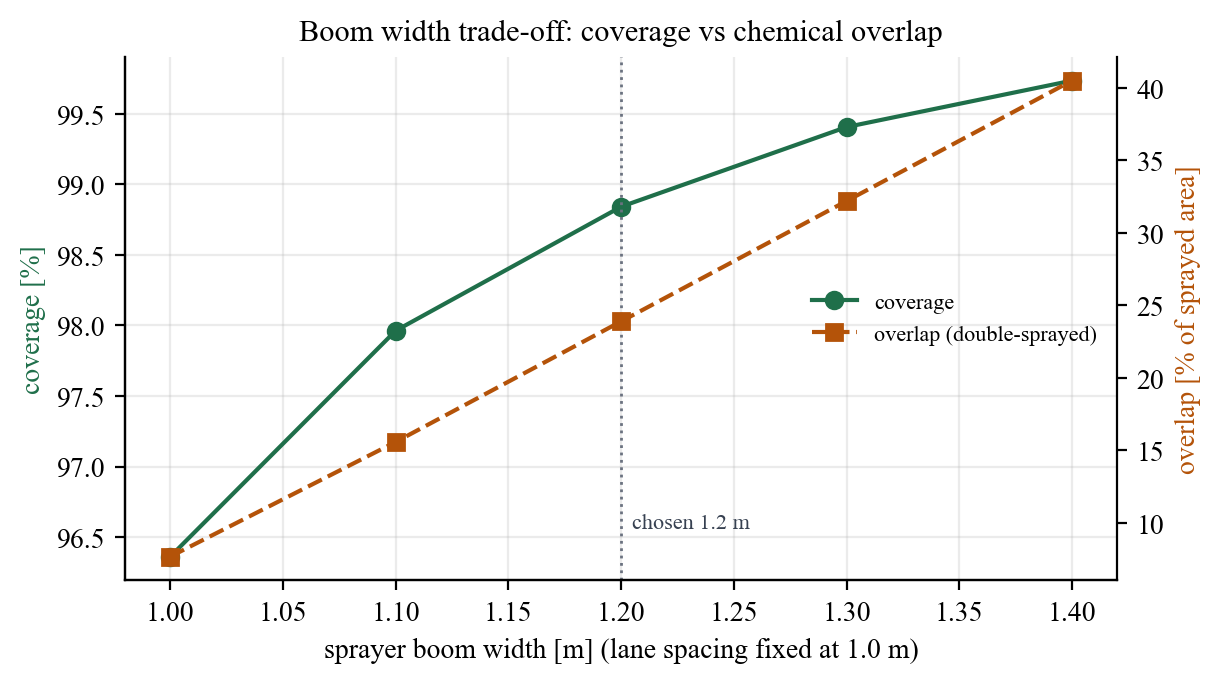
\includegraphics[width=\linewidth]{figures/fig_toolwidth.png}
\caption{Boom width trade-off}
\label{fig:toolwidth}
\end{minipage}\hfill
\begin{minipage}{0.41\linewidth}
\centering
\captionof{table}{Boom width study (20 fields)}
\label{tab:tool}
\renewcommand{\arraystretch}{1.15}
\small\begin{tabular}{|c|c|c|}
\hline
\textbf{Boom [m]} & \textbf{Cov. [\%]} & \textbf{Overl. [\%]} \\ \hline
1.0 & 96.36 & 7.7 \\ \hline
1.1 & 97.96 & 15.6 \\ \hline
\textbf{1.2} & \textbf{98.84} & \textbf{23.9} \\ \hline
1.3 & 99.41 & 32.2 \\ \hline
1.4 & 99.74 & 40.5 \\ \hline
\end{tabular}
\end{minipage}
\end{figure}

\subsection{Controller tuning (step response)}
Figure~\ref{fig:pid} and Table~\ref{tab:pid} show the lateral step responses used to tune the heading loop (Section~7.5). The chosen gains settle within the $\pm5$\,\% band in 2.9~s with 0.3\,\% overshoot, half the settling time of the low-gain setting. On the lanes this gives the 2.1~cm RMS cross-track error of Table~\ref{tab:mc}.

\begin{figure}[H]
\centering
\begin{minipage}{0.56\linewidth}
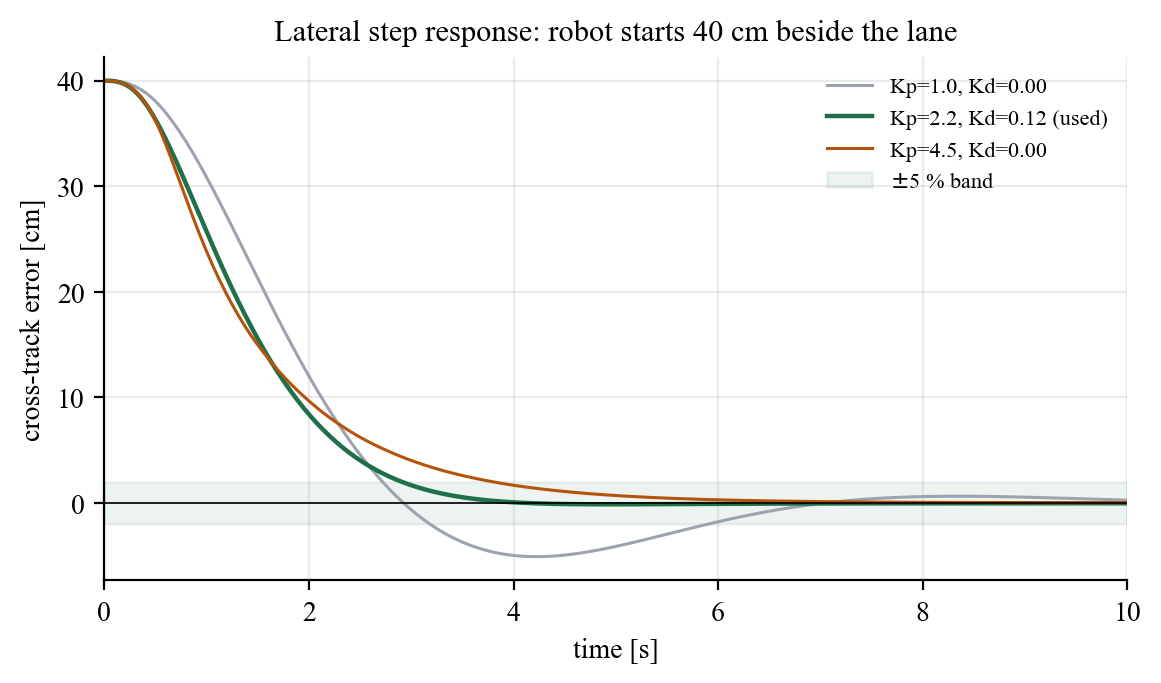
\includegraphics[width=\linewidth]{figures/fig_pid_step.png}
\caption{Lateral step response for three gain sets}
\label{fig:pid}
\end{minipage}\hfill
\begin{minipage}{0.41\linewidth}
\centering
\captionof{table}{Step-response metrics}
\label{tab:pid}
\renewcommand{\arraystretch}{1.15}
\small\begin{tabular}{|P{1.75cm}|c|c|c|}
\hline
\textbf{Gains} & \textbf{$t_r$ [s]} & \textbf{OS [\%]} & \textbf{$t_s$ [s]} \\ \hline
$K_p$=1.0 & 2.56 & 12.7 & 5.92 \\ \hline
$K_p$=2.2, $K_d$=0.12 & 2.53 & 0.3 & \textbf{2.91} \\ \hline
$K_p$=4.5 & 3.01 & 0.0 & 3.81 \\ \hline
\end{tabular}
\end{minipage}
\end{figure}

Figure~\ref{fig:timeline} shows the speed profile of the Webots run: the robot drives at 0.5~m/s on the lanes, slows to 0.3~m/s in headland turns and to about 0.2~m/s when a stone is ahead, then accelerates again along the detour arc.

\begin{figure}[H]
\centering
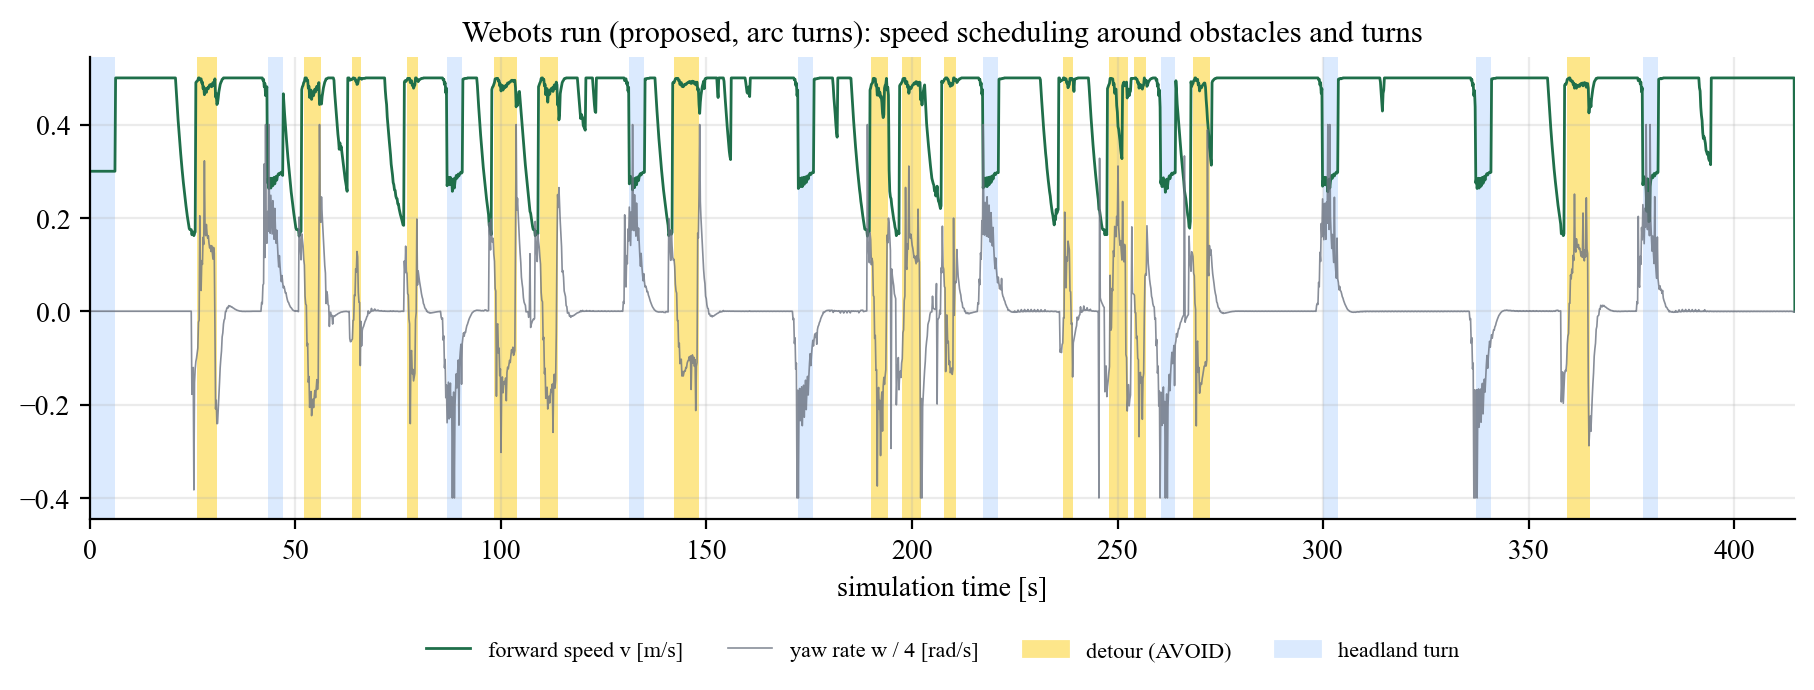
\includegraphics[width=\linewidth]{figures/fig_timeline.png}
\caption{Speed and yaw rate during the Webots run, with detours and turns highlighted}
\label{fig:timeline}
\end{figure}

\subsection{What worked and what did not}
\textbf{Worked.} Planning detours on a map instead of reacting to raw ranges kept the robot on its lane pattern: no lane segment was ever skipped by the proposed method. Running the same agent in Webots and in the headless simulator allowed fast statistics and gave consistent results (98.43 vs 98.97\,\% coverage on the demonstration field).

\textbf{Did not work at first.} (1) In Webots the first version became stuck in lane 5. The obstacle map contained 31 confirmed entries, 17 of them phantoms caused by single ghost returns at object edges; adding the isolated-return filter solved it. (2) Pure pursuit cut the inside of the detour arcs and passed a stone with only 1.8~cm clearance, which we fixed with the shorter detour look-ahead. (3) Redrawing the whole dashboard every update made Webots crash after about 400~s; incremental drawing fixed it. (4) APF needed a vortex term, a locked passing side and stall detection to finish most fields, and still failed 5 of 20.

\textbf{Limitations.} Obstacles are modelled as circles, so long obstacles (fences, ditches) would give large detours. Pose comes from ideal GPS. The lidar sees stones somewhat smaller at its mounting height, which is covered by the safety margin. The crop plants are not physical obstacles in simulation, so a detour may cross a neighbouring crop row. A real robot would choose the side that stays in the lane gap or straddle the row. The small triangular gaps just before and after each obstacle (Figure~\ref{fig:webots}) are the remaining 1.2\,\% of missed area.

\section{Contribution}
\renewcommand{\arraystretch}{1.5}
\begin{longtable}{|c|P{3.1cm}|P{7.0cm}|P{2.2cm}|}
\hline
\textbf{S. No.} & \textbf{Name and SAP ID} & \textbf{Technical contribution} & \textbf{Report sections + signature} \\ \hline
1 & Jahanvi Sengar (500120543) & Field and world design: \texttt{agri/field.py} (field model, random generator, JSON), \texttt{tools/generate\_world.py} (Webots world, robot extensions, sprayer boom, Pen), \texttt{tools/scenery.py} (lettuce, obstacles, farmyard, soil texture); Figures~\ref{fig:overview}, \ref{fig:robot}. & Abstract, 1, 2, 13 \\ \hline
2 & Aagman Sharma (500123462) & Coverage planning: \texttt{agri/planner.py} (boustrophedon path, arc and pivot headland turns, \texttt{Path} splicing), path statistics, arc vs pivot experiment (Section 9.3); report figure scripts \texttt{experiments/make\_figures.py} and \texttt{experiments/plotting.py}; Figure~\ref{fig:plan}. & 3, 4 \\ \hline
3 & Rudra Gupta (500120437) & Navigation and control: \texttt{agri/navigation.py} (PID, pure-pursuit tracker, speed scheduling, pivot hysteresis and lock), layered agent \texttt{agri/agent.py} (declarative, procedural and reflexive layers), Webots controller in \texttt{controllers/} (devices, wheel mapping, sprayer Pen, dashboard, logging), system integration, PID step-response tuning (Section 9.5); Figures~\ref{fig:pid}, \ref{fig:timeline}. & 5, 6 \\ \hline
4 & Sahil Agarwal (500120211) & Perception and avoidance: \texttt{agri/avoidance.py} (tilt and ghost filters, clustering, circle fit, obstacle map, geometric detour, Bug2 and APF baselines), slide generator \texttt{slides/make\_slides.py}; Figures~\ref{fig:perception}, \ref{fig:detour}. & 7, 8 \\ \hline
5 & Harsh Prakash Sinha (500123860) & Coverage logging and experiments: \texttt{agri/coverage.py}, \texttt{sim/headless\_sim.py}, \texttt{experiments/run\_experiments.py} and \texttt{experiments/run\_webots.py} (Monte-Carlo, density, boom width and Webots batch runs), result files in \texttt{results/}; Tables~\ref{tab:webots}--\ref{tab:tool}. & 9, 12, Appendix \\ \hline
\end{longtable}
\renewcommand{\arraystretch}{1.2}
All members took part in integration testing in Webots, the recorded presentation and the live demonstration. Each claim above can be traced to the member's commits in the GitHub repository.

\section{Co-learning Reflection}
\textbf{Jahanvi Sengar:} I learned on my own how Webots worlds, PROTO nodes and textures work, and how to generate a whole \texttt{.wbt} file from Python so that every field is reproducible from a seed. From Sahil I learned why the lidar sees stones smaller than they are, which changed how I placed the rocks. From Harsh I learned how the coverage grid is computed. I taught the team how to open, edit and reset the world, and how to add sensors to the Pioneer's extension slot.

\textbf{Aagman Sharma:} I studied coverage path planning papers and learned how lane spacing, overshoot and headland turns change the total path length and time. From Rudra I learned how the tracker uses the corner flags in my path to reduce its look-ahead at pivot points. From Sahil I learned how detours are spliced into the path, which led me to add duplicate-point removal to \texttt{Path.splice}. I explained the boustrophedon idea and the arc vs pivot trade-off to the team.

\textbf{Rudra Gupta:} I learned on my own how pure pursuit works, why it cuts corners, and how to tune a PID loop from a step response (rise time, overshoot, settling time). From Aagman I learned how the path is represented and tagged, and from Sahil how obstacle detection feeds into the tracker. From Harsh I learned how the cross-track error is measured. I taught the team the skid-steer wheel equations and why the pivot direction must be locked near 180 degrees.

\textbf{Sahil Agarwal:} I learned how a 2-D lidar works in Webots, how to cluster scans and fit circles, and what mixed-pixel ghost returns are and how to filter them. From Rudra I learned how the look-ahead distance affects clearance on curved detours. From Jahanvi I learned how the world is built, which helped me debug the phantom obstacles. I taught the team the APF and Bug2 algorithms we used as baselines and how to read the obstacle map dump.

\textbf{Harsh Prakash Sinha:} I learned how to design fair experiments (same seeds for every method, mean and standard deviation, worst case), run them in parallel and present them as box plots. From Aagman I learned the planner structure, and from Rudra the control parameters I swept. From Sahil I learned how the three avoidance methods differ, which helped me explain their failure cases. I taught the team how to run Webots in batch mode and regenerate all figures with one command.

\section{Conclusion and Future Scope}
We built a complete agricultural coverage robot in Webots that sprays a crop field lane by lane, maps unknown stones and poles with its lidar and avoids them with lane-preserving geometric detours. The robot finished every one of 20 random fields with 98.85\,\% coverage, no collisions and a cross-track error of 2.1~cm. Compared with Bug2 and a reactive potential field, it left 4--13 times less unsprayed area, was 13--47\,\% faster on average and never lost its lane. The design studies show that arc headland turns are 7.4\,\% faster than pivot turns and that a 1.2~m boom on 1~m lanes is a good balance between coverage and chemical overlap.

\textbf{Industrial use.} The same planner, tracker and detour logic suit spraying, mechanical weeding and scouting robots in row crops and orchards. Because the method keeps the lane pattern, the coverage map it logs can be used directly as a treatment record for precision agriculture. The reflexive stop layer matches the protective-stop requirement of ISO~18497.

\textbf{Moving to a real robot.} The \texttt{agri} package has no Webots dependency, so only the device layer must be replaced: RTK-GNSS and an IMU for the pose, a 2-D lidar driver (for example over ROS~2) for the ranges, and a motor driver for the wheel speeds. Future work: polygon obstacle models for long obstacles, localisation with sensor fusion instead of ideal GPS, crop-row-aware detour sides, uneven terrain, and replanning of the remaining lanes when several obstacles cluster together.

\begin{thebibliography}{99}
\addcontentsline{toc}{section}{References}
\setlength{\itemsep}{2pt}
\bibitem{vougioukas2019} S. G. Vougioukas, ``Agricultural robotics,'' \textit{Annual Review of Control, Robotics, and Autonomous Systems}, vol. 2, pp. 365--392, 2019.
\bibitem{grimstad2017} L. Grimstad and P. J. From, ``The Thorvald II agricultural robotic system,'' \textit{Robotics}, vol. 6, no. 4, p. 24, 2017.
\bibitem{bechar2016} A. Bechar and C. Vigneault, ``Agricultural robots for field operations: Concepts and components,'' \textit{Biosystems Engineering}, vol. 149, pp. 94--111, 2016.
\bibitem{choset2000} H. Choset, ``Coverage of known spaces: The boustrophedon cellular decomposition,'' \textit{Autonomous Robots}, vol. 9, no. 3, pp. 247--253, 2000.
\bibitem{galceran2013} E. Galceran and M. Carreras, ``A survey on coverage path planning for robotics,'' \textit{Robotics and Autonomous Systems}, vol. 61, no. 12, pp. 1258--1276, 2013.
\bibitem{oksanen2009} T. Oksanen and A. Visala, ``Coverage path planning algorithms for agricultural field machines,'' \textit{Journal of Field Robotics}, vol. 26, no. 8, pp. 651--668, 2009.
\bibitem{hameed2013} I. A. Hameed, D. Bochtis, and C. A. S{\o}rensen, ``An optimized field coverage planning approach for navigation of agricultural robots in fields involving obstacle areas,'' \textit{International Journal of Advanced Robotic Systems}, vol. 10, no. 5, 2013.
\bibitem{khatib1986} O. Khatib, ``Real-time obstacle avoidance for manipulators and mobile robots,'' \textit{The International Journal of Robotics Research}, vol. 5, no. 1, pp. 90--98, 1986.
\bibitem{koren1991} Y. Koren and J. Borenstein, ``Potential field methods and their inherent limitations for mobile robot navigation,'' in \textit{Proc. IEEE International Conference on Robotics and Automation}, Sacramento, CA, USA, 1991, pp. 1398--1404.
\bibitem{lumelsky1987} V. J. Lumelsky and A. A. Stepanov, ``Path-planning strategies for a point mobile automaton moving amidst unknown obstacles of arbitrary shape,'' \textit{Algorithmica}, vol. 2, pp. 403--430, 1987.
\bibitem{iso18497} \textit{Agricultural machinery and tractors --- Safety of highly automated agricultural machines --- Principles for design}, ISO 18497:2018, International Organization for Standardization, Geneva, Switzerland, 2018.
\bibitem{michel2004} O. Michel, ``Webots: Professional mobile robot simulation,'' \textit{International Journal of Advanced Robotic Systems}, vol. 1, no. 1, pp. 39--42, 2004.
\bibitem{brooks1986} R. A. Brooks, ``A robust layered control system for a mobile robot,'' \textit{IEEE Journal on Robotics and Automation}, vol. 2, no. 1, pp. 14--23, 1986.
\bibitem{coulter1992} R. C. Coulter, ``Implementation of the pure pursuit path tracking algorithm,'' Robotics Institute, Carnegie Mellon University, Pittsburgh, PA, USA, Tech. Rep. CMU-RI-TR-92-01, 1992.
\bibitem{astrom2008} K. J. {\AA}str{\"o}m and R. M. Murray, \textit{Feedback Systems: An Introduction for Scientists and Engineers}. Princeton, NJ, USA: Princeton University Press, 2008.
\bibitem{siegwart2011} R. Siegwart, I. R. Nourbakhsh, and D. Scaramuzza, \textit{Introduction to Autonomous Mobile Robots}, 2nd ed. Cambridge, MA, USA: MIT Press, 2011.
\bibitem{tuley2005} J. Tuley, N. Vandapel, and M. Hebert, ``Analysis and removal of artifacts in 3-D LADAR data,'' in \textit{Proc. IEEE International Conference on Robotics and Automation}, Barcelona, Spain, 2005, pp. 2203--2210.
\end{thebibliography}

\section*{Appendix: Links and Logs}
\addcontentsline{toc}{section}{Appendix: Links and Logs}
\textbf{GitHub repository:} \url{https://github.com/byRudra/AgriCoverageRobot_G11} \\[6pt]
\textbf{YouTube video (Unlisted):} \rule{8.3cm}{0.4pt}

\textbf{Meeting log}

\renewcommand{\arraystretch}{1.5}
\begin{tabular}{|c|P{1.9cm}|P{1.8cm}|P{2.2cm}|P{5.6cm}|}
\hline
\textbf{No.} & \textbf{Date} & \textbf{Duration} & \textbf{Attendees} & \textbf{Decisions} \\ \hline
1 & 24-Oct-2026 & 25 min & All 5 members & Roles and modules fixed; GitHub repository created; Webots + Pioneer 3-AT chosen \\ \hline
2 & 29-Oct-2026 & 30 min & All 5 members & Field size, lane spacing and boom width fixed; world generator and planner reviewed \\ \hline
3 & 03-Nov-2026 & 30 min & All 5 members & Tracker and PID gains reviewed; Bug2 and APF chosen as baselines \\ \hline
4 & 07-Nov-2026 & 20 min & All 5 members & Phantom-obstacle bug analysed; ghost and tilt filters added \\ \hline
5 & 11-Nov-2026 & 25 min & All 5 members & Experiment plan (20 seeds), report writing split and slide plan agreed \\ \hline
6 & 15-Nov-2026 & 30 min & All 5 members & Dry run of the 20-minute presentation and live demo \\ \hline
\end{tabular}
\renewcommand{\arraystretch}{1.2}

\vspace{6pt}
\textbf{Peer-assessment sheets} (each member fills one sheet for every team-mate; scores 1--5)

\renewcommand{\arraystretch}{1.25}
\small\begin{tabular}{|P{4.0cm}|C{2.2cm}|C{2.2cm}|C{2.2cm}|C{2.2cm}|}
\hline
\multicolumn{5}{|l|}{\textbf{Filled by:} Jahanvi Sengar (500120543) \quad \textbf{Signature:} \rule{3.5cm}{0.4pt}} \\ \hline
\textbf{Team-mate name and SAP ID} & \textbf{Contribution} & \textbf{Reliability / on time} & \textbf{Helped others learn} & \textbf{Quality of work} \\ \hline
Aagman Sharma (500123462) & 5 & 5 & 5 & 5 \\ \hline
Rudra Gupta (500120437) & 5 & 5 & 5 & 5 \\ \hline
Sahil Agarwal (500120211) & 5 & 5 & 5 & 5 \\ \hline
Harsh Prakash Sinha (500123860) & 5 & 5 & 5 & 5 \\ \hline
\end{tabular}
\normalsize
\renewcommand{\arraystretch}{1.2}

\vspace{8pt}
\renewcommand{\arraystretch}{1.25}
\small\begin{tabular}{|P{4.0cm}|C{2.2cm}|C{2.2cm}|C{2.2cm}|C{2.2cm}|}
\hline
\multicolumn{5}{|l|}{\textbf{Filled by:} Aagman Sharma (500123462) \quad \textbf{Signature:} \rule{3.5cm}{0.4pt}} \\ \hline
\textbf{Team-mate name and SAP ID} & \textbf{Contribution} & \textbf{Reliability / on time} & \textbf{Helped others learn} & \textbf{Quality of work} \\ \hline
Jahanvi Sengar (500120543) & 5 & 5 & 5 & 5 \\ \hline
Rudra Gupta (500120437) & 5 & 5 & 5 & 5 \\ \hline
Sahil Agarwal (500120211) & 5 & 5 & 5 & 5 \\ \hline
Harsh Prakash Sinha (500123860) & 5 & 5 & 5 & 5 \\ \hline
\end{tabular}
\normalsize
\renewcommand{\arraystretch}{1.2}

\vspace{8pt}
\renewcommand{\arraystretch}{1.25}
\small\begin{tabular}{|P{4.0cm}|C{2.2cm}|C{2.2cm}|C{2.2cm}|C{2.2cm}|}
\hline
\multicolumn{5}{|l|}{\textbf{Filled by:} Rudra Gupta (500120437) \quad \textbf{Signature:} \rule{3.5cm}{0.4pt}} \\ \hline
\textbf{Team-mate name and SAP ID} & \textbf{Contribution} & \textbf{Reliability / on time} & \textbf{Helped others learn} & \textbf{Quality of work} \\ \hline
Jahanvi Sengar (500120543) & 5 & 5 & 5 & 5 \\ \hline
Aagman Sharma (500123462) & 5 & 5 & 5 & 5 \\ \hline
Sahil Agarwal (500120211) & 5 & 5 & 5 & 5 \\ \hline
Harsh Prakash Sinha (500123860) & 5 & 5 & 5 & 5 \\ \hline
\end{tabular}
\normalsize
\renewcommand{\arraystretch}{1.2}

\vspace{8pt}
\renewcommand{\arraystretch}{1.25}
\small\begin{tabular}{|P{4.0cm}|C{2.2cm}|C{2.2cm}|C{2.2cm}|C{2.2cm}|}
\hline
\multicolumn{5}{|l|}{\textbf{Filled by:} Sahil Agarwal (500120211) \quad \textbf{Signature:} \rule{3.5cm}{0.4pt}} \\ \hline
\textbf{Team-mate name and SAP ID} & \textbf{Contribution} & \textbf{Reliability / on time} & \textbf{Helped others learn} & \textbf{Quality of work} \\ \hline
Jahanvi Sengar (500120543) & 5 & 5 & 5 & 5 \\ \hline
Aagman Sharma (500123462) & 5 & 5 & 5 & 5 \\ \hline
Rudra Gupta (500120437) & 5 & 5 & 5 & 5 \\ \hline
Harsh Prakash Sinha (500123860) & 5 & 5 & 5 & 5 \\ \hline
\end{tabular}
\normalsize
\renewcommand{\arraystretch}{1.2}

\vspace{8pt}
\renewcommand{\arraystretch}{1.25}
\small\begin{tabular}{|P{4.0cm}|C{2.2cm}|C{2.2cm}|C{2.2cm}|C{2.2cm}|}
\hline
\multicolumn{5}{|l|}{\textbf{Filled by:} Harsh Prakash Sinha (500123860) \quad \textbf{Signature:} \rule{3.5cm}{0.4pt}} \\ \hline
\textbf{Team-mate name and SAP ID} & \textbf{Contribution} & \textbf{Reliability / on time} & \textbf{Helped others learn} & \textbf{Quality of work} \\ \hline
Jahanvi Sengar (500120543) & 5 & 5 & 5 & 5 \\ \hline
Aagman Sharma (500123462) & 5 & 5 & 5 & 5 \\ \hline
Rudra Gupta (500120437) & 5 & 5 & 5 & 5 \\ \hline
Sahil Agarwal (500120211) & 5 & 5 & 5 & 5 \\ \hline
\end{tabular}
\normalsize
\renewcommand{\arraystretch}{1.2}

\end{document}
